\documentclass{article}
\usepackage[T1]{fontenc}
\usepackage[utf8]{inputenc}
\usepackage[ngerman]{babel}
\usepackage{graphicx}
\usepackage{geometry}
\usepackage{wrapfig}
\usepackage{tabularx}
\usepackage{subfigure} 
\usepackage{varwidth}
\usepackage{mwe}
\RequirePackage[ngerman=ngerman-x-latest]{hyphsubst}

\geometry{
	left=3cm,
	right=3cm,
	top=2cm,
	bottom=4cm,
	bindingoffset=5mm
}

\begin{document}
{\title{\Huge \textbf {Praxisbericht}}
\author{
\\
Zur betreuten Praxisphase\\
 im Bachelor Studiengang Angewandte Informatik\\
vom 1.März - 30. Juli 2018\\
bei\\
\\
PRÜFTECHNIK Condition Monitoring GmbH\\
Hähnlehofstraße 5. 88250 Weingarten\\
Betreuer: Dipl.-Ing. (FH) Siegfried Büchele
\\
\\
Fakultät Elektrotechnik und Informatik\\
Hochschule Ravensburg-Weingarten\\
Studiengang Angewandte Informatik\\
Doggenriedstrasse\\
88250 Weingarten \\
\\
\\
\\
Maximilian Nestle (27427)\\
Wilhelmstraße 41\\
88250 Weingarten\\
\\
 }
\date{\today}
\maketitle
 \newpage
\tableofcontents 
\newpage

\section{Tagesberichte} 
	\begin{tabular}{l|p{2.5cm}|p{15cm}}
	{\large Tag} &{\large  Wochentag, Datum }& {\large Tätigkeit in Stichworten} \\	& & \\
	
 		& & \\
		& \textbf{Woche 1}&\\


		1 & Do 01.03.2018 & 
			Einführung, Tablet einrichten, Android Media Recorder \\

		2 & Fr 02.03.2018	 & 
			Tonaufnahme. Audio Storage einrichten\\
	

		& \textbf{Woche 2}&\\

		
		3 & Mo 05.03.2018	 & 
			Inbetriebnahme ,,Testinput-Gerät'', Datenvisualisierung mit Excel\\


	
		4 & Di 06.03.2018 & 
			Empfangen von Daten des Frequenzgenerators\\

	
		5 & Mi 07.03.2018 & 
			Verschiedene Abtastraten, Shell Scripts, Frequenz Sweep\\

	
		6 & Do 08.03.2018 & 
			GUI Verbesserung, Recorder Objekt, GraphViewer \\

	
		7 & Fr 09.03.2018 & 
			Datenanzeige mit Zoom und Scale, 2. Datenanzeige für FFT Daten\\
			

		& \textbf{Woche 3}&\\

	
		8 & Mo 12.03.2018 & 
			Android NDK: einbinden der fftw Bibliothek(C++), Build mit cmake\\

	
		9 & Di 13.03.2018 & 
			FFT Java Bibliothek, Fensterfunktion, imaginär und real Anteil verrechnen \\

		
		10 & Mi 14.03.2018 & 
		FFT und Fenster Funktion verbessert\\

		
		11 & Do 15.03.2018  & 
		Speicher/Buffer Verwaltung, GUI Timepicker, Dropdown Menu\\

		12 & Fr 16.03.2018 & 
		 Activity für die Graphanzeige, FFT Daten speichern\\
		 

		 & \textbf{Woche 4}&\\

		 
		 13 & Mo 19.03.2018	 & 
		 Dämpfung ausgleichen, Stopp Recording \\

		 
		 14 & Di 20.03.2018	 & 
		 Anzeigen min/max, Hochpass, APK erstellen und testen\\

		 15 & Mi 21.03.2018 & 
		 Vergleich zwischen Smartphone und Tablet, Encoding Test \\

		 16 & Do 22.03.2018 & 
		 Recherche PCM 16/24 Bit\\

		 17 & Fr 23.03.2018 & 
		 Weitere Recherchen: Smartphone mit 24 Bit AD Wandler\\


		& \textbf{Woche 5}&\\

		
		
		18 & Mo 26.03.2018 & 
			Anfertigen der Projektdokumentation\\

		19 & Di 27.03.2018	 & 
		Projektdokumentation, XML output, realer Sensor\\

		20 & Mi 28.03.2018 & 
			Messungen mit Rotorkit\\

		21 & Do 29.03.2018 & 
			Weitere Messungen, Dämpfungsfunktion verbessern\\

		 & Mi 14.03.2018 & 
			Karfreitag\\

		

		& \textbf{Woche 6}&\\

		
		
		& Mo 02.04.2018  & 
		Ostermontag\\

		22 & Di 03.04.2018	 & 
		2. Projekt (Verlust von Formaten), Einarbeiten\\

		23 & Mi 04.04.2018	 & 
		Verschiedene Encoder (mp3, ogg), Präsentation für Projekt 1\\

		24 & Do 05.04.2018 & 
		FLAC Encoder/Decoder\\

		25 & Fr 06.04.2018 & 
		Encoden mit SoX und ffmpeg\\

		& \textbf{Woche 7}&\\

		
		
		26 & Mo 09.04.2018  & 
		Erfolgreiches Encoden mit SoX (flac) ogg teilweise\\

		27 & Di 10.04.2018  & 
		.cvs in .XML, Encoden von realen Messergebnissen\\

		28 & Mi 11.04.2018		 & 
		FFT Vergleich: vor Komprimierung – nach Komprimierung \\

		29 & Do 12.04.2018 & 
		SoX kompilieren, Versuch Zeitmessung.\\

		30 & Fr 13.04.2018 & 
		mp3 Encoder\\

				

		& \textbf{Woche 8}&\\

		31 & Mo 16.04.2018	  & 
		Dokumentation Projekt 2, Tests\\

		32 & Di 17.04.2018  & 
		Dokumentation/ Präsentation von Projekt 1 und 2\\

		33 & Mi 18.04.2018	 & 
		Tests mit verschiedenen Dateigrößen\\

		34 & Do 19.04.2018 & 
		Präsentation und Dokumentation. Code Refactoring\\

		35 & Fr 20.04.2018 & 
		Code Refactoring (Kommentare) mp3 Encoding bzw. Decoding\\

	
	\end{tabular}
	\begin{tabular}{l|p{2.5cm}|p{15cm}}
		

		& \textbf{Woche 9}&\\

		
		
		36 & Mo 23.04.2018	  & 
		Projekt Nr. 3, JavaFX, seriellen Verbindung\\

		37 & Di 24.04.2018  & 
		COM senden/empfangen, Test mit VIBGUARD compact\\

		38 & Mi 25.04.2018	 & 
		Java http Client\\

		39 & Do 26.04.2018 & 
		Senden/speichern der Einstellungen, Einstellungen von Webserver\\

		40 & Fr 27.04.2018 & 
		Automatisches Detektieren der IP Adresse, Username/Password\\


		& \textbf{Woche 10}&\\

		
		
		41 & Mo 30.04.2018	  & 
		Gleitzeit\\

		 & Di 01.05.2018	  & 
		Tag der Arbeit\\

		42 & Mi 02.05.2018	 & 
		IP Adressen Eingabe, Ant make Builder\\

		43 & Do 03.05.2018 & 
		 Batch File zum Ausführen der jar Datei\\

		44 & Fr 04.05.2018 & 
		IP Validierung, XML Templates mit Hilfe von Drag and Drop.\\

		
	\end{tabular}
	\begin{tabular}{l|p{2.5cm}|p{15cm}}
		

		& \textbf{Woche 11}&\\

		
		
		45 & Mo 07.05.2018	  & 
		Speichern eines Templates, Gateway Validierung.\\

		46& Di 08.05.2018	  & 
		Anwendungsbetrieb ohne serielle Verbindung, Race Condition\\

		47 & Mi 09.05.2018		 & 
		Scheduler, Stoppen des Schreibvorgangs\\

		& Do 10.05.2018  & 
		Christi Himmelfahrt\\

		48 & Fr 11.05.2018 & 
		Gleitzeit\\


		& \textbf{Woche 12}&\\

		
		
		49 & Mo 14.05.2018	  & 
		Pings über C Interpreter, Info Tab\\

		50 & Di 15.05.2018	  & 
		Umbau der GUI, Integrieren von Tooltips\\

		51 & Mi 16.05.2018		 & 
		Tooltips, Usability, Standard Templates, .jar in .exe \\

		52 & Do 17.05.2018  & 
		Login Dialog, Buttons zum Speichern und Öffnen der Templates\\

		53 & Fr 18.05.2018 & 
		Abbruchmanagement, Refactoring\\


		& \textbf{Woche 13}&\\

		
		& Mo 21.05.2018	  & 
		Pfingstmontag\\

		54 & Di 22.05.2018	  & 
		Test mit VIBROWEB XP (Monitoring Device) JRE 8 -> JRE 6\\

		
		55 & Mi 23.05.2018		 & 
		Realer Test, Ändern der Syntax auf Java 7, Dialogklasse\\

		56 & Do 24.05.2018  & 
		Java 7 Dialoge, Intefaceanpassung, Java Version auf 1.7.0.65\\

		57 & Fr 25.05.2018 & 
		Testen der 1.7.0.65 Version, Windows Installers mit Hilfe\\
	

	
			

			& \textbf{Woche 14}&\\

			
			
			58 & Mo 28.05.2018	  & 
			Verbessern des Installers- Auto Start nach Installation, Dokumentation.\\

			59 & Di 29.05.2018	  & 
			Hilfetexte im Footer, Ladeanzeige (JavaFX Animation)\\

			60 & Mi 30.05.2018			 & 
			 Ladeanimation ein- bzw. ausblenden, Error Handling\\

			 & Do 31.05.2018  & 
			Fronleichnam\\

			61 & Fr 01.06.2018 & 
			Gleitzeit\\

			

			& \textbf{Woche 15}&\\

			
			
			62 & Mo 04.06.2018	  & 
			Test mit VIBROWEB XP und Java 1.7.0.60, Fertigstellung des Programms\\

			63 & Di 05.06.2018	  & 
			Erstellen einer „Aufbau“ Grafik zum einfacheren Verständnis\\

			64 & Mi 06.06.2018			 & 
			 Projekt 4, React Js, webpack, babel und development Server\\

			65 & Do 07.06.2018  & 
			Toolbar, Swipe View, Appbar\\

			66 & Fr 08.06.2018 & 
			Redux, resonsive UI\\

			

			& \textbf{Woche 16}&\\

			
			
			67 & Mo 04.06.2018	  & 
			Fortsetzen der Arbeit Responsivity, Anfang erster Tab (GUI)\\

			68 & Di 05.06.2018	  & 
			Power saving Tab Unit tab redux\\

			69 & Mi 06.06.2018			 & 
			Seal/Bearing/Pump Tab, bundled.js Optimierung\\

			70 & Do 07.06.2018  & 
			Einheiten der Textfelder, Snackbar für Ergebnisse\\

			71 & Fr 08.06.2018 & 
			Dialogfenster für die  Zusammenfassung der Ergebnisse\\
			
			
	\end{tabular}
	\begin{tabular}{l|p{2.5cm}|p{15cm}}



			& \textbf{Woche 17}&\\

			
			
			72 & Mo 18.06.2018	  & 
			Responsive, Hinzufügen der Werteberechnung\\

			73 & Di 19.06.2018	  & 
			Buggfix (Swipe), Werteberechnung vom Original übernehmen.\\

			74 & Mi 20.06.2018			 & 
			Werteberechnung, Dialog für Best Case	\\

			75 & Do 21.06.2018  & 
			Dialog Inhalt für ''Best Case Example''\\

			76 & Fr 22.06.2018 & 
			Werteberechnung für Best Case Dialog\\

			

			& \textbf{Woche 18}&\\
		
			
			77 & Mo 18.06.2018	  & 
			Performance Verbesserungen, Einarbeitung in Cookieverwaltung\\

			78 & Di 19.06.2018	  & 
			GUI Umgestaltung für mobile Geräte\\

			79 & Mi 20.06.2018			 & 
			Layout auf Grid Layout\\

			80 & Do 21.06.2018  & 
			Best Case umstellen auf Grid Layout. Ergebnisfeld auf Hauptseite\\

			81 & Fr 22.06.2018 & 
			Design Anpassung \\
			

			& \textbf{Woche 19}&\\
		
		
			& Mo 02.07.2018	  & 
			Begleitseminar zum Praxissemester\\

			& Di 03.07.2018	  & 
			Begleitseminar zum Praxissemester\\

			79 & Mi 04.07.2018			 & 
			Design und Performance\\

			80 & Do 05.07.2018  & 
			React Hash Router\\

			81 & Fr 06.07.2018 & 
			Design Finish, Bericht\\
			
	

			& \textbf{Woche 20}&\\
			
			
			85 & Mo 09.07.2018  & 
			HTML und WebApp Manifest\\

			86 & Di 10.07.2018	  & 
			SSL Zertifikat erstellen\\

			87 & Mi 11.07.2018			 & 
			https und ServiceWorker\\

			88 & Do 12.07.2018  & 
			Icons, Bericht\\

			89 & Fr 13.07.2018 & 
			LaTex, Bericht\\


			& \textbf{Woche 21}&\\

			
			90 & Mo 16.07.2018  & 
			LaTex installieren und einarbeiten\\

			91 & Di 17.07.2018	  & 
			Praxisbericht\\

			92 & Mi 18.07.2018			 & 
			Praxisbericht\\

			93 & Do 19.07.2018  & 
			Praxisbericht\\

			94 & Fr 20.07.2018 & 
			Praxisbericht\\

			


			& \textbf{Woche 22}&\\

			
			
			95 & Mo 23.07.2018  & 
			Anleitung zu Projekt 4, GIT, Praxisbericht\\

			96 & Di 24.07.2018	  & 
			Praxisbericht\\

			97 & Mi 25.07.2018	 & 
			Praxisbericht\\

			98 & Do 26.07.2018  & 
			Praxisbericht\\

			99 & Fr 27.07.2018 & 
			Praxisbericht\\

			


			& \textbf{Woche 23}&\\

				
			100 & Mo 30.07.2018  & 
			Praxisbericht\\




		
	\end{tabular}

\newpage


\section{Das Unternehmen}
	\subsection{Generell}

		PRÜFTECHNIK ist ein mittelständisches Unternehmen mit ungefähr 600 Mitarbeitern, das im Jahr 1972 von Dieter Busch gegründet wurde. Der Hauptsitz liegt in Ismaning bei München. Die Firma besitzt zudem noch diverse Zweigstellen, wobei eine in Weingarten angesiedelt ist.\\
		PRÜFTECHNIK stellt hauptsächlich Geräte zur Überwachung und Ausrichtung von Maschinen her. Die Maschinenausrichtung und Vermessung wird mit Hilfe von Lasern realisiert, die hochpräzise gebaut und ausgerichtet werden müssen. \\


	\subsection{Weingarten}
		Die in Weingarten hergestellten Geräte gehören zu dem Bereich der Online Condition Monitoring Geräte.
		Merkmal dieser Systeme ist, dass sie die Sensordaten dauerhaft auswerten und dann über das Internet an die jeweilige Auswertungsstelle senden.\\ Diese Geräte werden in Weingarten entwickelt und auch gefertigt.

	\subsection{Produkte}


\section{Kurzbeschreibung der Aufgaben/Projekte während der Praxisphase}
	\subsection{Auslesen von Sensordaten mit Hilfe eines Android Smartphones} 

		Mit Hilfe eines Android Smartphones oder Tablet sollen Sensordaten ausgelesen werden. Dazu soll der analoge Mikrofoneingang benutzt werden um einen Sensor anzuschließen.\\
		Aufgabe in diesem Projekt ist es, eine App zu entwickeln, die diese Daten ausliest, anzeigt und weiterleitet.

	\subsection{Vergleich verschiedener Komprimierungsarten} 

		Bei den Online Monitoring Systemen der Firma PRÜFTECHNIK werden täglich sehr viele Daten erzeugt und versendet. Nicht immer ist aber eine geeignete Internetverbindung gegeben. Dabei wäre es wünschenswert die Daten zu komprimieren.\\
		Aufgabe ist nun, bekannte Audiokomprimierungsverfahren darauf zu prüfen, ob sie die Daten verkleinern können ohne zu viele Informationen zu verlieren.

	\subsection{Gerätekonfigurator über COM Port} 

		Die Monitoring Geräte, die mit dem Internet verbunden sind, verwenden oft einen Webserver um Einstellungen vorzunehmen. Stellt man aber aus Versehen die falschen Netzwerkparameter ein, ist der Webserver nicht mehr erreichbar. Für diesen Fall besitzen die Geräte eine serielle Schnittstelle, über die man ebenfalls konfigurieren kann. Aufgabe ist es, die sehr benutzerunfreundliche Kommandoeingabe durch eine GUI zu ersetzen, um das Zurück- bzw. Neusetzen der Einstellungen so einfach wie möglich zu machen.

	\subsection{WebApp: Return of Investment} 

		Ein ,,Return of Investment'' Rechner soll dem Kunden zeigen, wie er langfristig mit dem Kauf eines Produktes Geld einsparen kann. Für die ,,Alignment'' Geräte hat PRÜFTECHNIK so einen Rechner. Dieser Rechner soll neu als WebApp realisiert werden, so dass er auf allen Endgeräten einsetzbar ist.



\section{Projekt 1: Auslesen von Sensordaten mit Android} 
	\subsection{Motivation/Aufgabe}
		Die von PRÜFTECHNIK gebauten mobilen „Datensammler“, wie zum Beispiel der VIBSCANNER 2 , sind im Industriestandard gebaut und dafür ausgelegt möglichst schnell Schwingungsdaten zu erfassen. Dabei werden die Sensordaten ausgelesen, verarbeitet, gespeichert und später weitergegeben.
		Theoretisch müsste ein modernes Smartphone oder Tablet auch in der Lage sein diese Aufgaben zu erledigen.
		Natürlich wären die Messdaten bei weitem nicht so genau, jedoch für Veranschaulichung/Marketing Zwecke wären sie ausreichend. Zudem ist der finanzielle Aspekt und die Tatsache, dass fast jeder dauerhaft ein Smartphone bei sich trägt nicht zu vernachlässigen.

	\subsection{Android}
		Android ist ein von Google verwaltetes Betriebssystem, das mit einem Marktanteil von 74,8 Prozent die Smartphone Welt in Deutschland dominiert. Dabei handelt es sich um eine Open Source Software, die auf einen Linux Kernel aufbaut. Zum Programmieren von Android Applikationen kann entweder Java oder Kotlin verwendet werden. Zudem kann auch ein NDK (Native Development Kit) eingesetzt werden um C und C++ Code einzubetten. In diesem Projekt wurde aber ausschließlich Java verwendet.

		\subsubsection{Android Studio}
			Android Studio ist die bei diesem Projekt eingesetzte Entwicklungsumgebung. Sie basiert auf der IntelliJ IDEA und ist die offizielle Entwicklungsumgebung für Android.

		\subsubsection{Android Schnittstellen}
			Android bietet eine Vielzahl verschiedener Schnittstellen (APIs), die es möglich machen auf Geräteeigenschaften, Funktionen aber auch Informationen zuzugreifen. Hierbei ist zu beachten, dass die APIs abhängig von einem API- Level sind, das bei jeder neuen Android Version hochgezählt wird. So darf das API-Level auf dem Android Device (z.B. Android 6.0 API- Level 23) nicht kleiner sein als das Minimum API- Level der gewünschte API.

	\subsection{Programmieren einer Android Applikation}
		\subsubsection{Activity}

			\begin{wrapfigure}[16]{r}[0pt]{0.5\textwidth}
				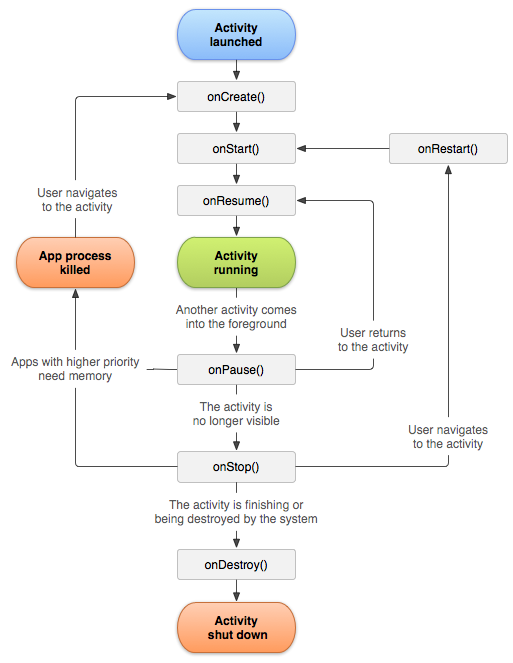
\includegraphics[scale=0.35]{Bilder/activity_lifecycle.png}
				\centering
				\vspace{0 cm}
				\caption{Activity Lebenszyklus}
				\label{fig1}	
			\end{wrapfigure}


			Eine Activity ist eine Bildschirmseite einer Android App. Eine App kann aus beliebig vielen Activities bestehen. Einer Activity kann ein Layout zugeordnet werden, das dann auf dem Bildschirm angezeigt wird. Eine Activity ist eine Java Klasse, die von der Klasse andoid.app.Activity abgeleitet wird.
			Eine Activity besitzt einen Lebenszyklus (Activity-lifecycle) der immer durchlaufen wird. In \textit{Abbildung \ref{fig1}} sind die verschiedenen Status einer Activity dargestellt. Die Funktionen, wie zum Beispiel onCreate(), werden dann aufgerufen, wenn die entsprechende Stelle im Lebenszyklus erreicht wurde.
			Um von einer Activity zur nächsten zu wechseln werden Intents verwendet, die auch dazu benutzt werden können um Variablen zu übergeben.

		\subsubsection{Layout}
			Bei Android wird das Layout von einer XML Datei beschrieben. Diese beinhaltet die verschiedenen GUI Objekte. Die Layout Datei kann entweder von Hand oder mit Hilfe eines Interfaces erstellt werden. Zusätzlich kann man den XML Code auch während der Laufzeit verändern.

		\subsubsection{Gradle}
			Gradle ist für das „Bauen“ einer App zuständig. In der build.gradle Datei wird festgelegt, welche Android Version benutzt werden soll aber auch welche zusätzlichen Bibliotheken eingebunden werden sollen.

		\subsubsection{Android Manifest}
			In dieser XML Datei werden die Einstellungen der App festgelegt, wie zum Beispiel der Name der App, die benutzten Activities und auch die Berechtigungen, die die App benötigt.

		\subsubsection{Debuggen}
			Android bietet zum Debuggen die Android Debug Bridge (adb), mit der man auf das mit USB verbundene Gerät zugreifen kann und es möglich macht die Log-Files einzusehen. Darüber hinaus lässt sich auch gleich die App auf das Handy übertragen. Optional kann man die App auch in einer Virtuellen Maschine öffnen.

	\subsection{Benutzte Schnittstellen und Bibliotheken}

		\subsubsection{Audio Record}
			AudioRecord ist eine Java Klasse, die es möglich macht mit der Smartphone Hardware Audio Daten aufzunehmen. Dabei hat sie den Vorteil, dass sie in der Lage ist Audiodateien im PCM (Puls-Code-Modulation) Format aufzunehmen. Das Encoding kann entweder auf 8/16 Bit oder float eingestellt werden. AudioRecord bietet auch eine frei wählbare Sample Rate an, die jedoch über 4000Hz und unter 19200Hz sein muss. Die Audio Quelle ist auch einstellbar, wobei hier die Einstellung UNPROCESSED die besten Ergebnisse bringt. Leider ist diese Einstellung erst ab dem API- Level 24 verfügbar, was die Hardware Auswahl weiter einschränkt.

		\subsubsection{Graph Viewer}
			Graph Viewer ist eine Open Source Bibliothek die es möglich macht, in Android Graphen zu zeichnen und diese als GUI Elemente hinzuzufügen. Hierbei muss die .jar Bibliothek in das Android Projekt eingebunden werden und der Graph Viewer ins Layout XML übernommen werden.

		\subsubsection{TarosDSP}
			Die Bibliothek TarosDSP ist eine Audioverarbeitungs-Bibliothek die es möglich macht, FFT Daten zu berechnen.

	\subsection{Hardware und Elektronik}


		\subsubsection{Android Device}
			Das für das Projekt hauptsächlich benutzte Android Gerät ist das Acer Iconia One 10 b3-a40 (Tablet). Zu Testzwecken wurden aber auch andere Android Smartphones und Tablets getestet.



		\subsubsection{Mikrophon Simulator}
			\begin{wrapfigure}[16]{r}[0pt]{0.5\textwidth}
				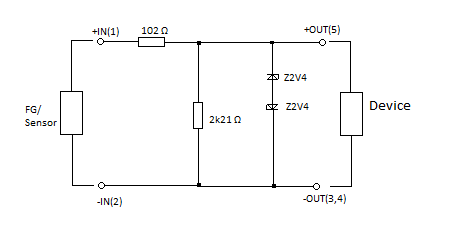
\includegraphics[scale=0.8]{Bilder/Schaltplan.png}
				\centering
				\vspace{0 cm}
				\caption{Schaltplan Mikrofon Simulator}
				\label{fig2}	
			\end{wrapfigure}

			Der „Mikrofon Simulator“ ist das Verbindungsstück zwischen Device und Signalquelle. Er wird benötigt, damit das jeweilige Android Device ein externes Mikrofon erkennt, obwohl eigentlich eine andere Signalquelle (z.B. Sensor oder Frequenzgenerator) angeschlossen ist.
			Dazu wird mit Widerständen die Impedanz eines Mikrophones simuliert. Ohne den Simulator würde das Smartphone oder Tablet das interne Mikrofon verwenden.
			Als Eingang dient ein AUX Kabel, das mit einem Klinken Stecker mit dem Device verbunden werden kann. Der Ausgang ist ein Koaxialkabel mit einer BNC-Steckverbindung, die mit einem Frequenzgenerator verbunden werden kann.\\
			In \textit{Abbildung \ref{fig2}} ist der elektronische Schaltplan zu sehen.

		\subsubsection{Frequenzgenerator}
			Frequenzgenerator zur Generierung eines konstanten (meist sinusförmigen) Signals. Dient als Testinput und zur Generierung von Referenzwerten.
			(Der hier verwendete Generator ist von der Firma Rohde \& Schwarz).

		\subsubsection{Sensor}

			Um die Vibrationen zu messen, werden Beschleunigungssensoren verwendet. In diesem Projekt wird einer vom Typ VIB 7.205 benutzt.

	\subsection{Ergebnisse}
		\subsubsection{Frequenzgang}

				In jedem Android Device ist ein Hoch- und Tiefpass integriert, der die Frequenzen beschränkt.
				Der Hochpass dämpft die niedrigen Frequenzen. Der 3 dB Punkt, des verwendeten Tablets, liegt bei 340Hz. 

				\begin{wrapfigure}[9]{r}[0pt]{0.5\textwidth}
					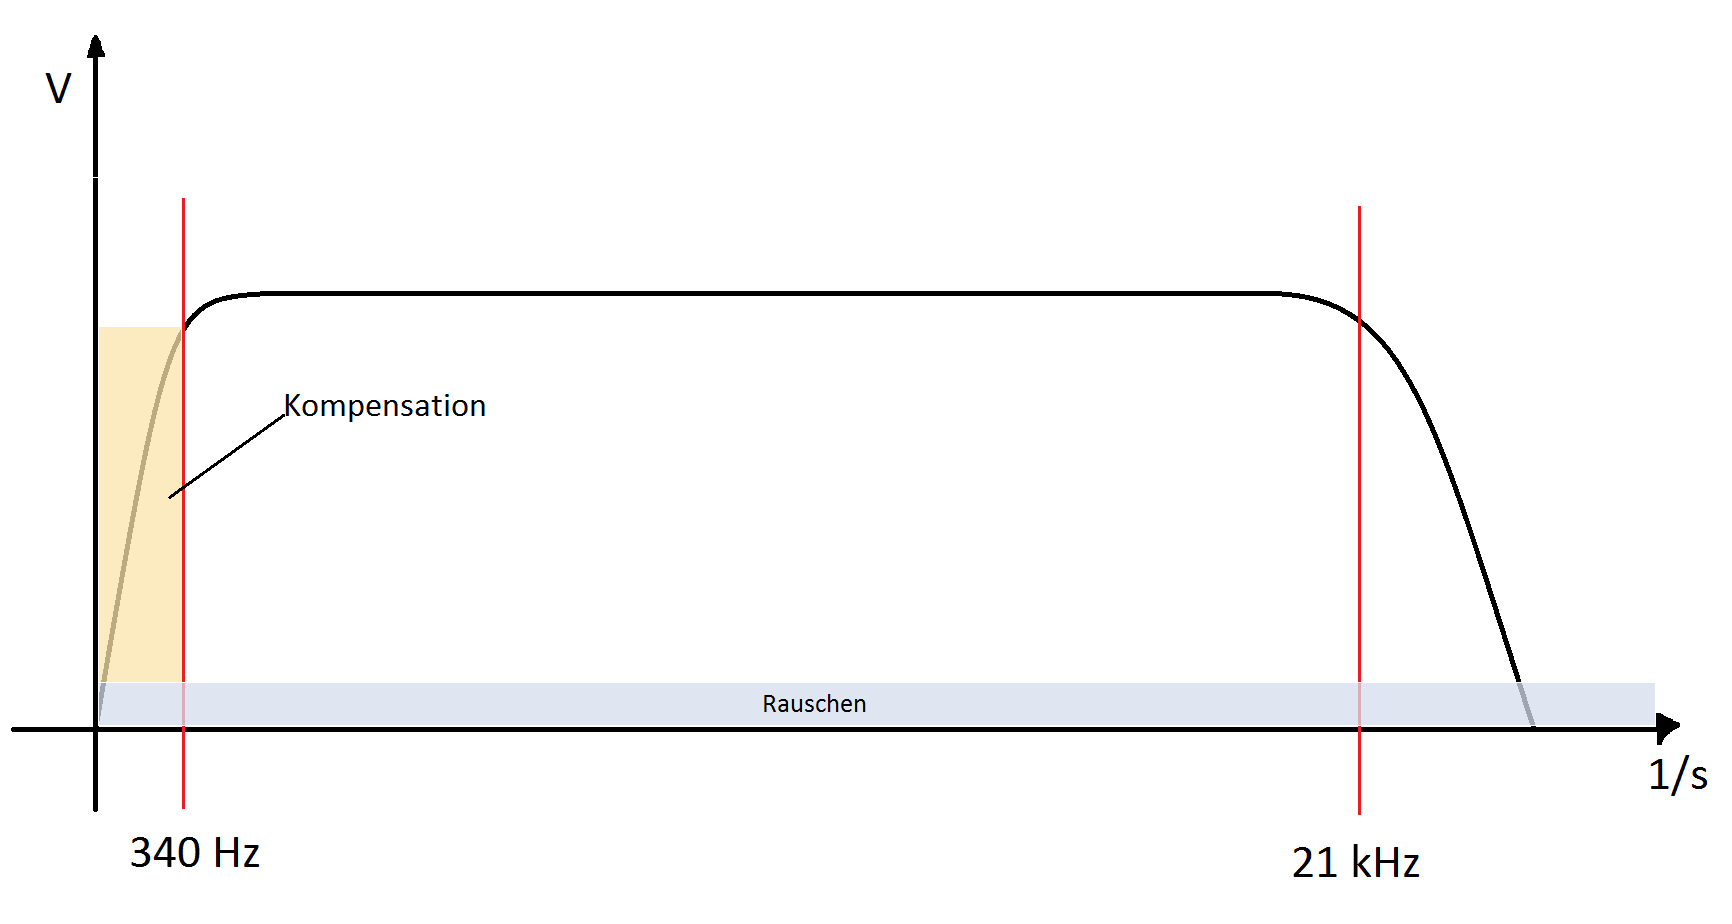
\includegraphics[scale=0.2]{Bilder/Frequenzgang.png}
					\centering
					\vspace{0 cm}
					\caption{Frequenzgang}
					\label{fig3}	
				\end{wrapfigure}

				Dieser Dämpfung kann mit Hilfe einer Korrekturfunktion entgegengewirkt werden. Nachteil hierbei ist aber, dass das Rauschen durch diese Funktion ebenfalls verstärkt wird. Darum wird die Korrekturfunktion erst dann angewendet, wenn die Amplitude höher als das Rauschen ist. Die Werte, die sich im Rauschbereich befinden, gehen aber verloren.
				Der Tiefpass dämpft die hohen Frequenzen. In diesem Fall liegt der 3 dB Punkt bei ungefähr 21 kHz, mehr ist bei einem Audioeingang auch eigentlich nicht nötig, da das menschliche Gehör höhere Frequenzen nicht wahrnehmen kann.


		\subsubsection{Messwerte}

				\begin{figure}[ht]
					\centering
					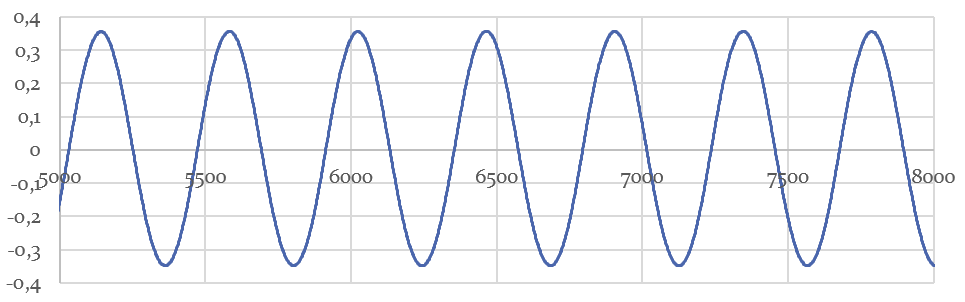
\includegraphics[scale=0.5]{Bilder/Mesurement-Best.PNG}
					\caption{Endergebnis bei mittlerer Frequenz}
					\label{fig4}
				\end{figure}

				\begin{figure}[ht]
					\centering
					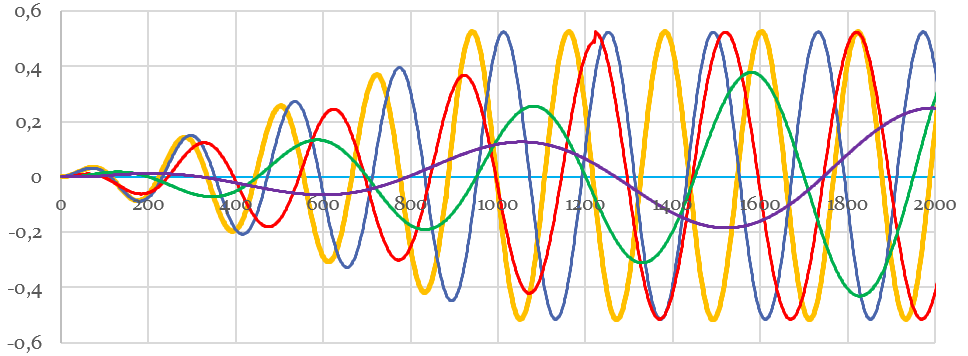
\includegraphics[scale=0.5]{Bilder/Messureent_SampleRate.PNG}
					\caption{Endergebnis bei verschiedenen Sample Raten}
					\label{fig5}
				\end{figure}
				
				\begin{figure}[ht]
					\centering
					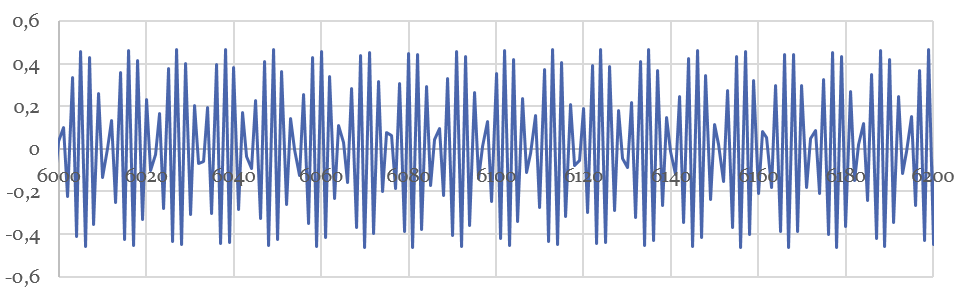
\includegraphics[scale=0.5]{Bilder/Messurement-tooHeigh.PNG}
					\caption{Endergebnis bei zu hoher Frequenz}
					\label{fig6}
				\end{figure}

\newpage

		\subsubsection{Vergleich VIBGUARD und Android}

					\begin{wrapfigure}[16]{r}[0pt]{0.5\textwidth}
						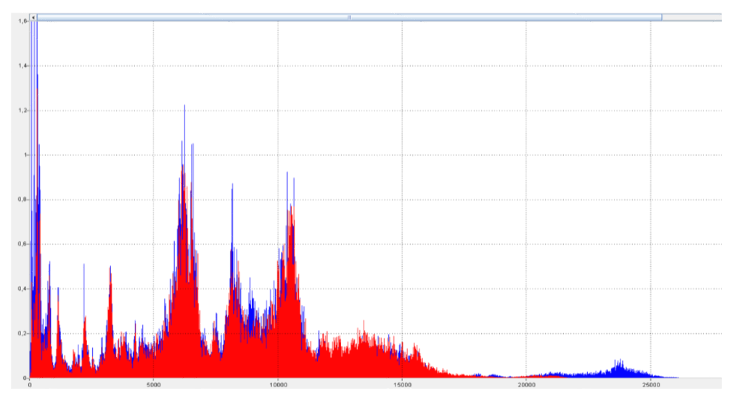
\includegraphics[scale=0.5]{Bilder/vergleich.png}
						\centering
						\vspace{0 cm}
						\caption{Vergleich VIBGUARD (blau) und Android}
						\label{fig7}	
					\end{wrapfigure}

					In \textit{Abbildung \ref{fig7}} ist der Vergleich zwischen einer Sensormessung mit einem VIBGUARD (blau) und der Messung mit einem Android Device (rot) zu sehen. Der benutzte Sensor ist ein Beschleunigungssensor (VIB 7.205) und ist an einem Rotor Kit angeschlossen. Dabei sind sich die beiden Daten im unteren bis mittleren Frequenzband sehr ähnlich. Bei hohen Frequenzen filtert der Tiefpass im Android Device ab ungefähr 22kHz die Frequenzen heraus.


	\subsection{Fazit/Zusammenfassung}
					Dafür, dass mit einem Smartphone die Sensordaten eingelesen worden sind, sind die Ergebnisse sehr zufriedenstellend. Mit Ausnahme sehr hoher Frequenzen über 20kHz sind die Daten beim VIBGUARD und bei der Android Messung sehr ähnlich.
					Wenn die hohen Frequenzen nicht zwingend benötigt werden, ist die App auch in der Lage reale Messungen durchzuführen.
					Für Demozwecke und zur Veranschaulichung kann die App auf jeden Fall genutzt werden.\\
					Ein großes Problem ist jedoch, dass sich die verschiedenen Smartphones sehr stark unterscheiden und es dadurch nahezu unmöglich ist, eine genaue Aussage über die Güte der gelesenen Daten zu machen. Außerdem wird von den Smartphone Herstellern fast nie angegeben, welcher AD- Wandler eingebaut ist. Leider ist meistens nicht mal bekannt, ob es sich um ein 16 oder 24 Bit AD-Wandler handelt.

	\subsection{Code}

		\subsubsection{Aufbau}
			\begin{wrapfigure}[12]{r}[0pt]{0.6\textwidth}
				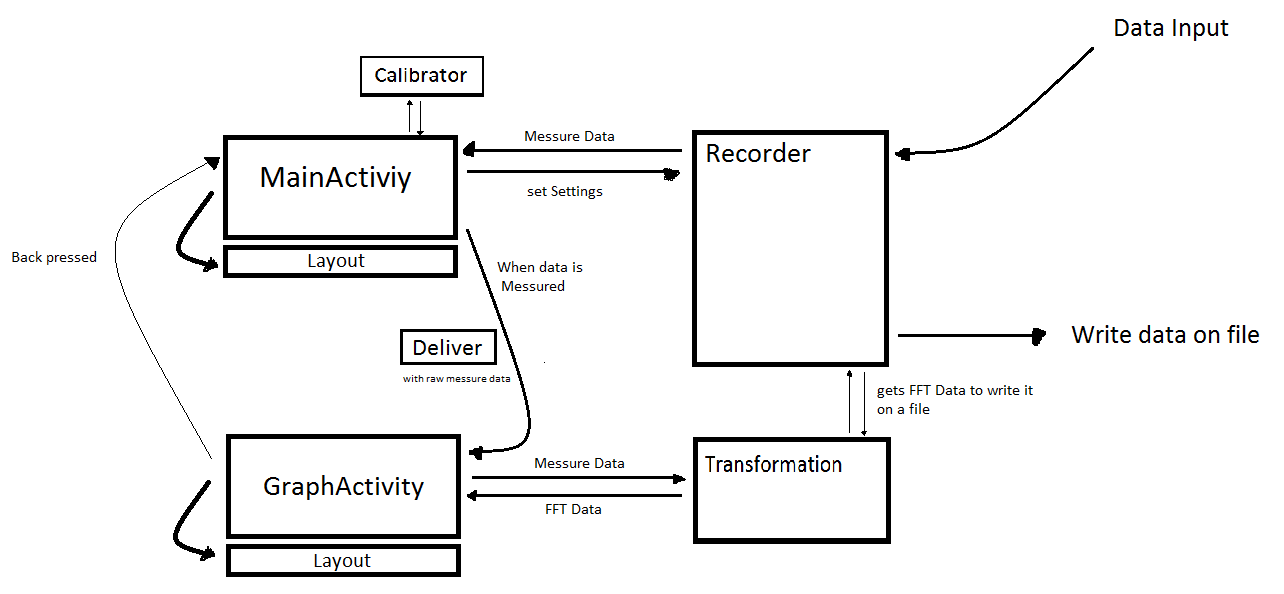
\includegraphics[scale=0.3]{Bilder/blockschaltbild.png}
				\centering
				\vspace{0 cm}
				\caption{Code Struktur}
				\label{fig8}	
			\end{wrapfigure}
			
			In \textit{Abbildung \ref{fig8}} ist der grobe Aufbau der Codestruktur verdeutlicht. Beim Starten der Application wird die MainActivity gestartet. Über die GUI können dann Einstellngen für den Recorder getroffen werden und ihn schließlich auch starten. Wenn die Daten gemessen sind, wird eine neue Activity (GraphActivity) gestartet, die die Messdaten auf dem Display darstellt. Die FFT Daten können über das Transformations Objekt berechnet werden.



\newpage
		\subsubsection{GUI}

		\begin{wrapfigure}[19]{r}[0pt]{0.6\textwidth}
			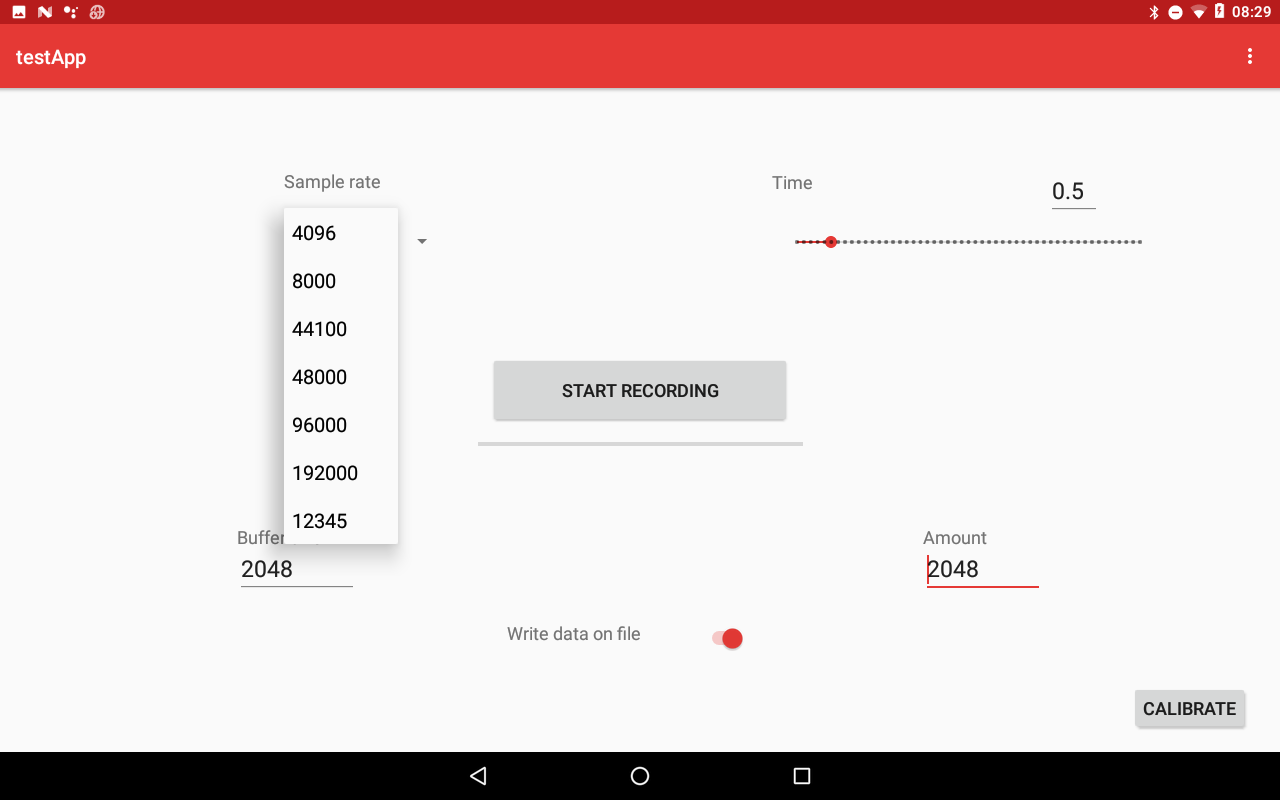
\includegraphics[scale=0.15]{Bilder/Screenshot_20180327-082929.png}
			\centering
			\vspace{0 cm}
			\caption{Main Layout}
			\label{fig9}	
		\end{wrapfigure}
	

	
		
			In \textit{Abbildung \ref{fig9}} ist das Layout der MainActivity zu sehen, welches es möglich macht, Einstellungen für den Recorder zu treffen. Mit Hilfe einer SeekBar kann die gewünschte Aufnahmezeit eingestellt werden. Die Auswahl der Sample Rate wird durch einen Spinner realisiert. Die Buffergröße und die Gesamtanzahl der Messdaten können bei Bedarf manuell angepasst werden, wobei dies nur selten der Fall ist. Mit dem ,,Calibrate'' Button kann die Kalibrierung (Berechnung des Offsets) gestartet werden. Wichtig dabei ist, dass am Eingang keine Spannung angelegt ist. Mit einem Switch kann nun noch entschieden werden, ob die gelesenen Daten auf eine Datei geschrieben werden sollen oder nicht. 
			
			\begin{wrapfigure}[16]{r}[0pt]{0.6\textwidth}
				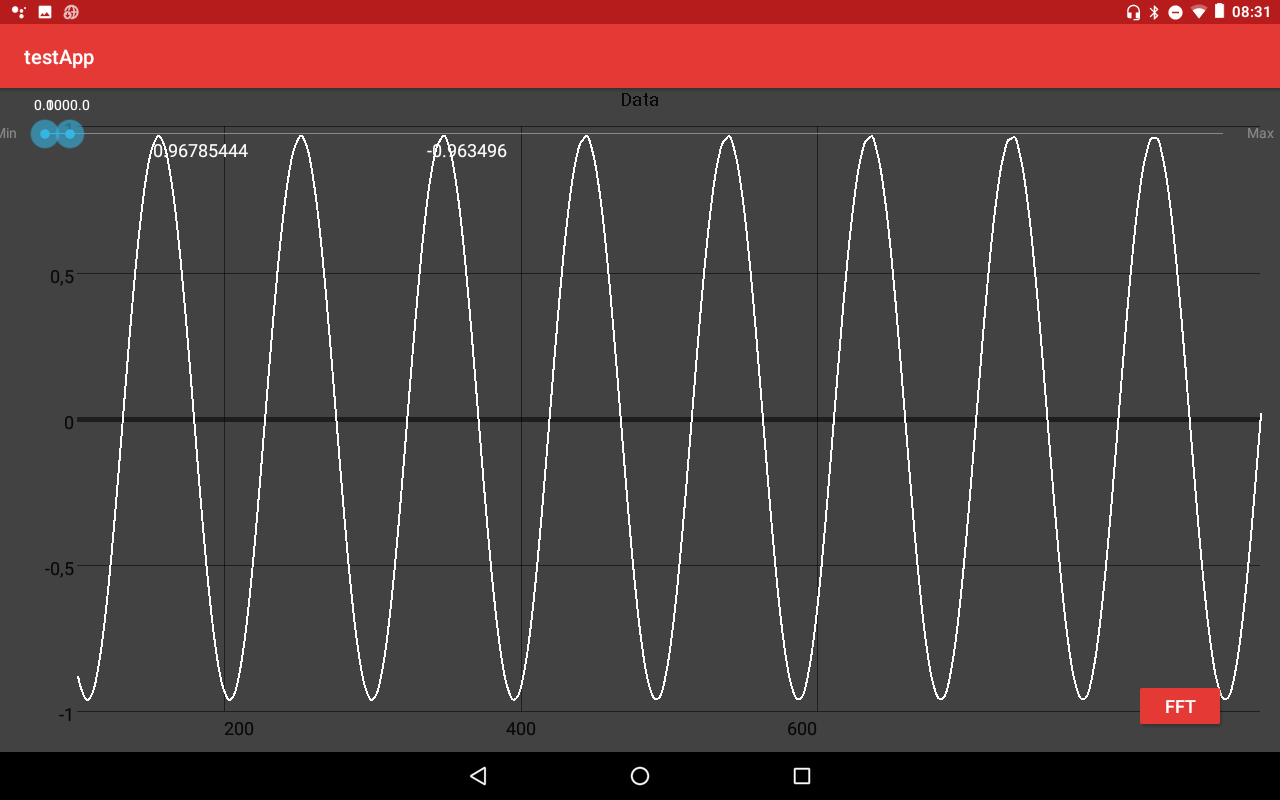
\includegraphics[scale=0.15]{Bilder/Screenshot_20180327-083120.png}
				\centering
				\vspace{0 cm}
				\caption{Graph/Daten Layout}
				\label{fig10}	
			\end{wrapfigure}
		
		
			
			Mit dem Start Button wird nun die Messung begonnen. Über eine ProgressBar kann man den Status der Messung nachvollziehen.
			
			\begin{wrapfigure}[16]{r}[0pt]{0.6\textwidth}
				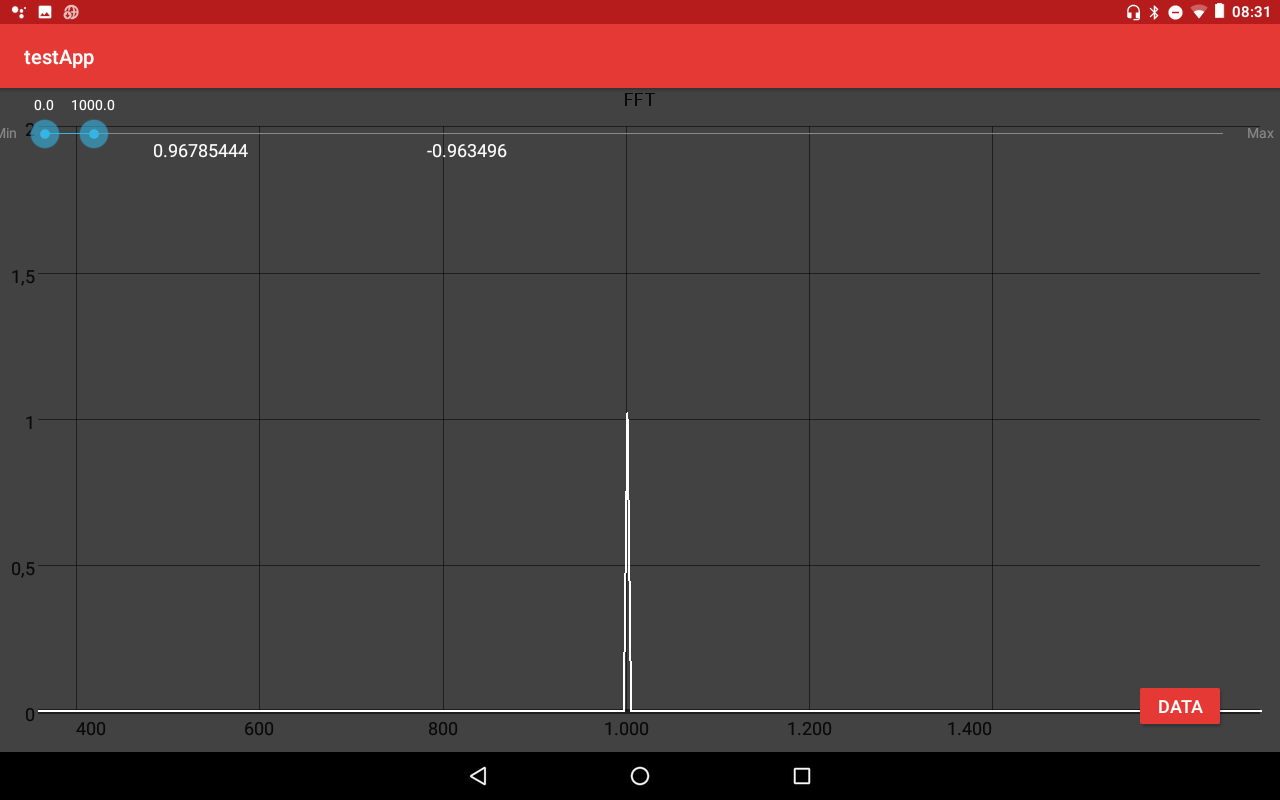
\includegraphics[scale=0.15]{Bilder/Screenshot_20180327-083144.png}
				\centering
				\vspace{0 cm}
				\caption{FFT Layout}
				\label{fig11}	
			\end{wrapfigure}
			
			Sind die Messdaten fertig so wird die GraphActivity gestartet und die Messdaten, wie in \textit{Abbildung \ref{fig10}}, angezeigt. Durch Klicken auf den FFT Button werden die FFT Daten angezeigt (\textit{Abbildung \ref{fig11}}).
			Eine RangeSeekBar, im oberen Teil der Anzeige, übernimmt die Auswahl des gewünschten Datenausschnittes.
			Wird die Android „Zurück Taste“ gedrückt so kommt man wieder auf die MainActivity.
			Als Layout wurde überall das Constraint Layout verwendet.
		
\newpage
	\subsection{Technische Begriffserklärung}
		\subsubsection{FFT}
						Kommt aus dem Englischen für „Fast Fourier Transform“. Die FFT ist ein Algorithmus, der das digitale Signal in seine Frequenzanteile zerlegt.

		\subsubsection{AD Wandler}
						Ein AD Wandler ist ein Analog Digital Wandler. Er hat als Input ein analoges Signal und liefert einen digitalen Wert zurück. Die gelieferten Werte können eine unterschiedliche Größe haben (z.B. 8 Bit 16 Bit oder 24 Bit). Umso höher der Bit Wert, umso genauer ist der AD Wandler und die resultierende Granularität.

		\subsubsection{PCM}
			PCM (Puls-Code-Modulation) ist ein unkompliziertes Audio Format, das aus einem zeitkontinuierlichen Signalverlauf eine zeitdiskrete Signalfolge generiert. Das bedeutet, dass in einer bestimmten Frequenz der Wert des analogen Signals in einen digitalen Wert umgewandelt und abgespeichert wird.

\section{Projekt 2: Kompression von Sensordaten} 
	\subsection{Einleitung}
		\subsubsection{Motivation}
			Die Condition Monitoring Geräte der Firma PRÜFTECHNIK produzieren viele Zeitsignale, deren Umfang leicht mehrere 100 MB pro Tag bedeuten können. Diese Daten müssen häufig über das mobile Netz (z.B. UMTS) übertragen werden. Dabei spielt das Datenvolumen eine große Rolle, da nicht unendlich Up- bzw. Download zur Verfügung steht.
		\subsubsection{Fragestellung}
			Ist es möglich die Messdaten mit Audiokompressionsverfahren zu komprimieren und zu dekomprimieren mit einem vertretbaren Verlust?	
	\subsection{Benutzte Werkzeuge}
		\subsubsection{Eclipse}
			Eclipse ist eine freie IDE. In diesem Projekt wird sie zum Programmieren des Java Codes verwendet.
		\subsubsection{Visual Studio 2010}
			Visual Studio ist eine IDE von Microsoft die benötigt wird, um aus dem SoX Source Code ein ausführbares Programm zu generieren.
		\subsubsection{SoX}
			SoX (Sound eXchange) ist ein Multifunktionswerkzeug zum Lesen und Schreiben von Audiodateien. Außerdem bringt SoX viele Encoder und Decoder mit sich, die es möglich machen die verschiedenen Dateiformate in andere umzuwandeln. SoX ist ein Open Source Projekt und kann von jedem verwendet werden.
		\subsubsection{TarsosDSP}
			TarsosDSP ist eine Java Bibliothek für Audio Verarbeitung. Sie ist außerdem in der Lage ein FFT zu berechnen, wozu sie in diesem Projekt ausschließlich verwendet wird.
	\subsection{Benutzte Formate}
		\subsubsection{Comma-Seperated Values (.cms)}
			Einfaches Dateiformat, bei dem die Werte in ASCII Codierung durch ein Komma getrennt gespeichert werden können. Wird hier dazu verwendet reale Messdaten zu importieren.
		\subsubsection{Extensible Markup Language (.xml)}
			Hierarchisch strukturiertes Dateiformat, das von Menschen und Maschinen gelesen werden kann. Hier wird es verwendet, um die Daten an ein Darstellungsprogramm (Pro Report) zu übergeben.
		\subsubsection{RAW-Daten (.raw)}
			Dieses Format enthält nur die binären Rohdaten ohne Verwendung eines Headers. (Im Code auch manchmal als PCM- Daten bezeichnet)
		\subsubsection{Wave-Dateiformat (.wav)}
			RAW-Daten aber mit Header.
		\subsubsection{Vorbis Ogg (.ogg)}
			Vorbis ist ein Audio-Codec der Xiph.Org Foundation. Die mit Vorbis codierten Dateien werden in einem Ogg Container gespeichert. Vorbis ist ein patentfreies Verfahren zur verlustbehafteten Audiodatenreduktion. Dabei basiert Vorbis wie mp3 oder AAC auf der Modifizierten Diskreten Kosinustransformation (MDCT), welche blockweise angewendet wird.
			Zusätzlich werden psychoakustische Effekte der Wahrnehmung ausgenutzt, wie zum Beispiel, dass hohe Frequenzen, die für das menschliche Gehör nicht wahrnehmbar sind, abgeschnitten werden.
			
		\subsubsection{Free Lossless Audio Codec (.flac)}
			FLAC (Free Lossless Audio Codec) ist ein Codec zur verlustfreien Audiokomprimierung. Der wie Vorbis von der Xiph.Org Foundation entwickelt wurde. Da FLAC eine verlustfreie Komprimierung ist, hat man keine Qualitätseinbußen, das heißt, dass (fast) keine Informationen verloren gehen (Rohdaten und Enddaten sind nahezu identisch).
			Dabei werden die Daten in Blöcke eingeteilt und die Werte mit einer Polynomfunktion dargestellt. Der Unterschied zwischen der Polynomfunktion und dem tatsächlichen Signal wird zusätzlich als Fehlersignal gespeichert.
			
	\subsection{Vorbis Komprimierung}	
		\subsubsection{Messdaten}
			Die Messdaten kommen von einem Beschleunigungssensor, der an einer Vakuumpumpe montiert ist.
			Die binären Rohdaten der Messung haben eine Größe von 5.242.880 Bytes (131072 Hz Sample Rate, 10 Sekunden, 32 Bit float).\\
			Ablauf:\\
			Rohdaten –- (Vorbis Codieren) --> .ogg Datei –-(Vorbis Decodieren) --> Enddaten\\\\
			Anmerkung: Die Rohdaten und die Enddaten haben die gleiche Größe, aber nicht den gleichen Informationsgehalt!
			
		
		\subsubsection{Zeit Daten}
		
			\begin{figure}
				
				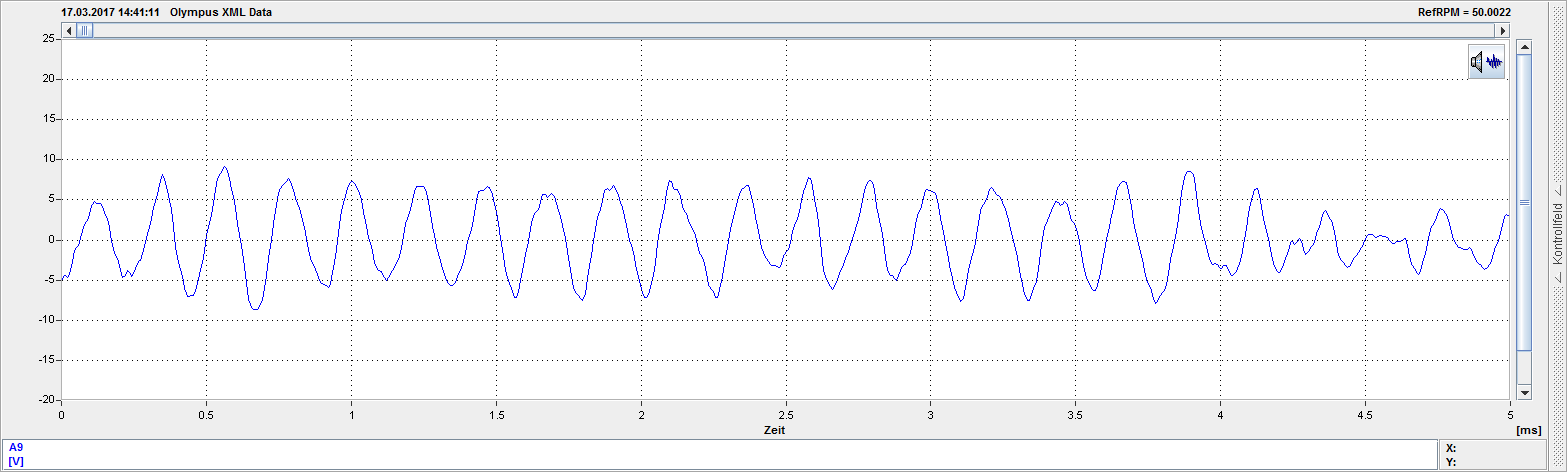
\includegraphics[scale=0.4]{Bilder/1.png}
				\centering
				\vspace{0 cm}
				\caption{Original Daten}
				\label{fig12}	
				
				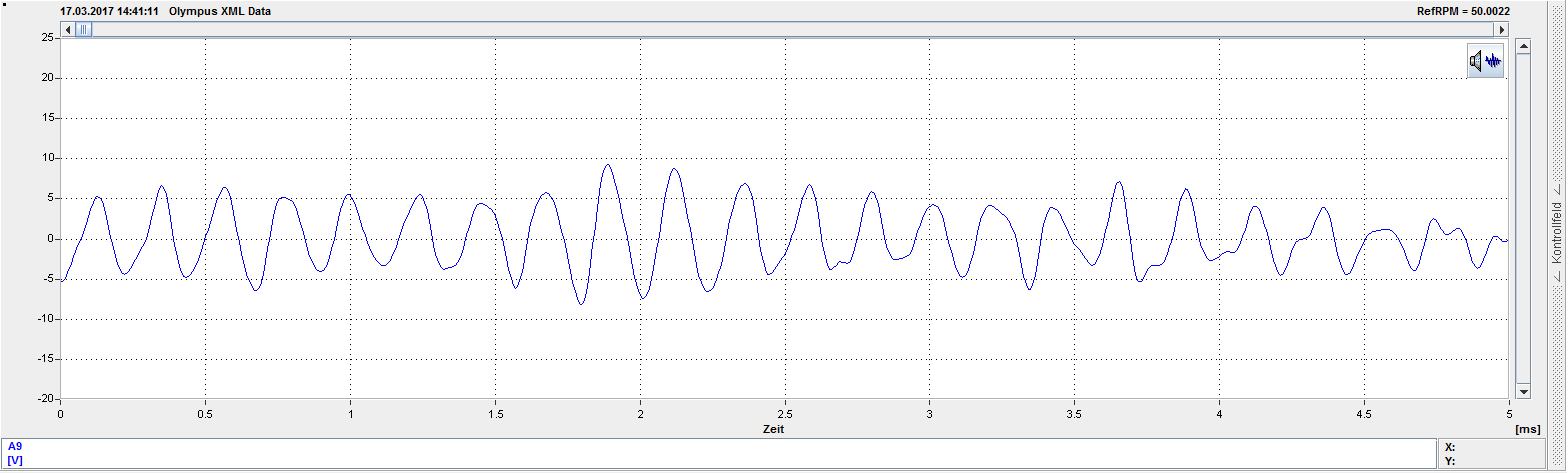
\includegraphics[scale=0.4]{Bilder/2.png}
				\centering
				\vspace{0 cm}
				\caption{Qualitätslevel -1}
				\label{fig13}	
				
				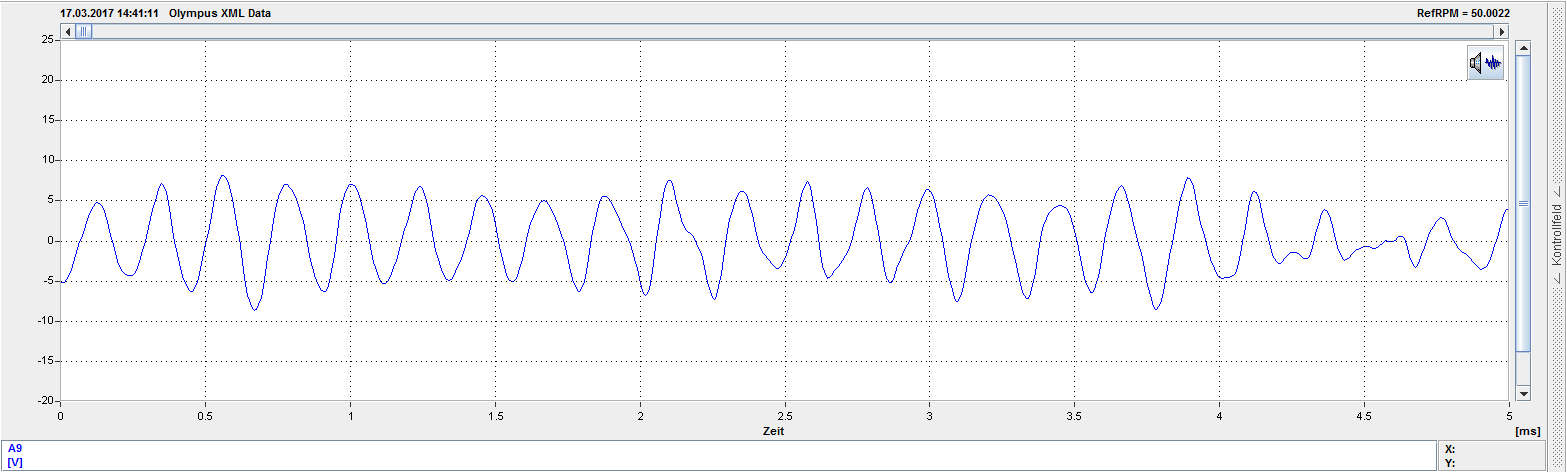
\includegraphics[scale=0.4]{Bilder/3.png}
				\centering
				\vspace{0 cm}
				\caption{Qualitätslevel 5}
				\label{fig14}	
				
				
				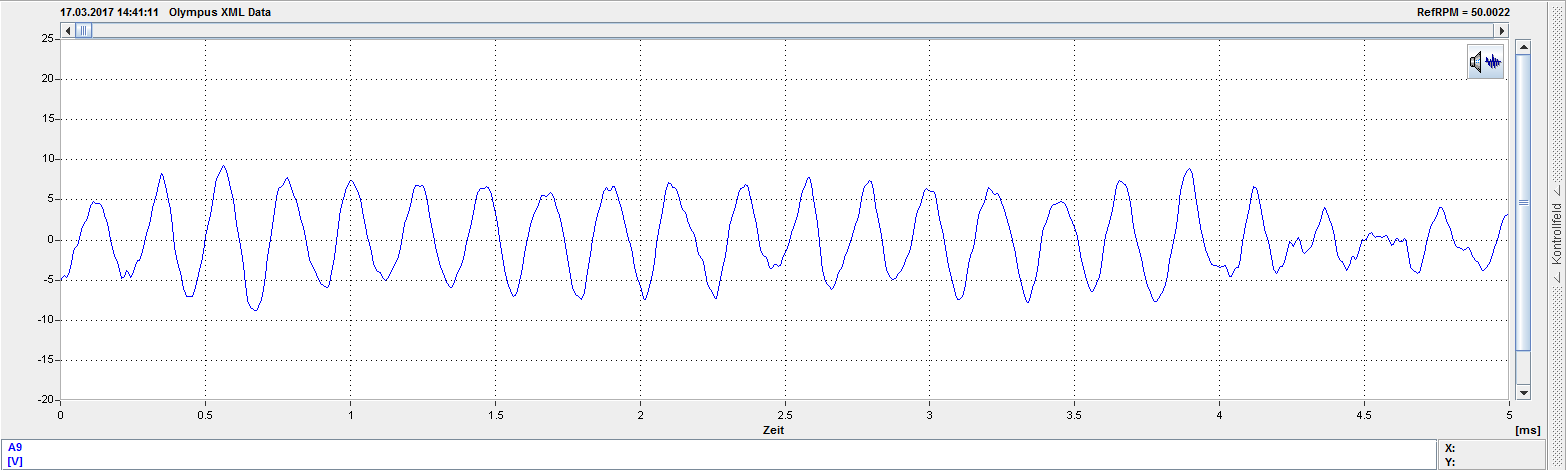
\includegraphics[scale=0.4]{Bilder/4.png}
				\centering
				\vspace{0 cm}
				\caption{Qualitätslevel 10}
				\label{fig15}
		
		\end{figure}
	
	
		\begin{figure}

			\begin{varwidth}[t]{\linewidth}
				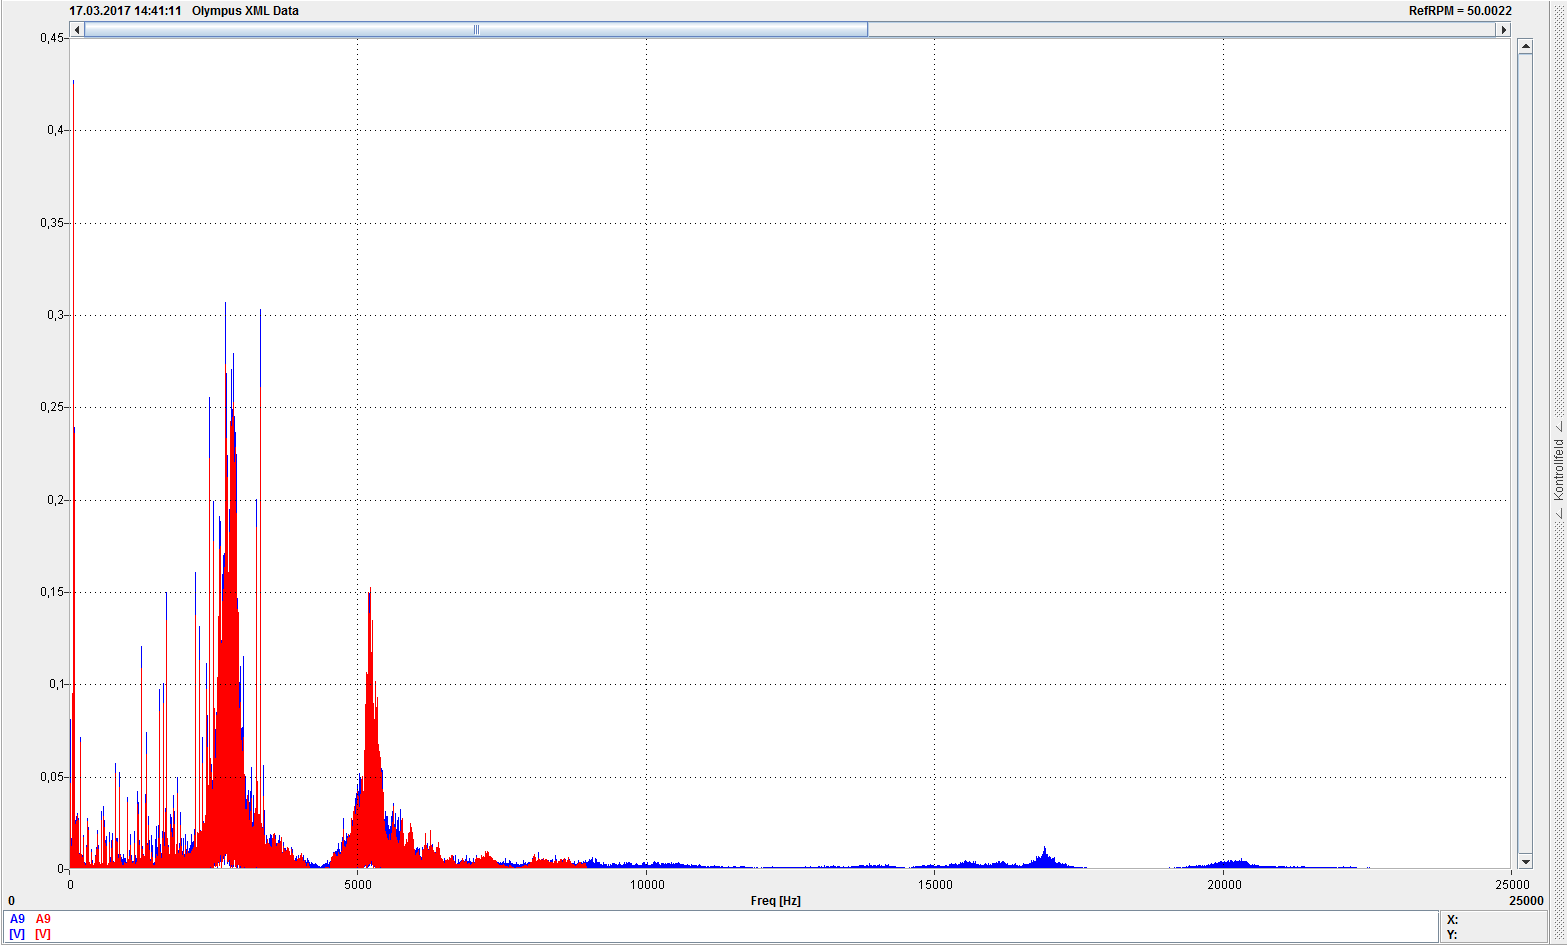
\includegraphics[width=0.49\textwidth]{Bilder/5.png}
				\caption{Qualitätslevel -1}
				\label{fig30}	
			\end{varwidth} % ein Leerzeichen Abstand
			\begin{varwidth}[t]{\linewidth}
				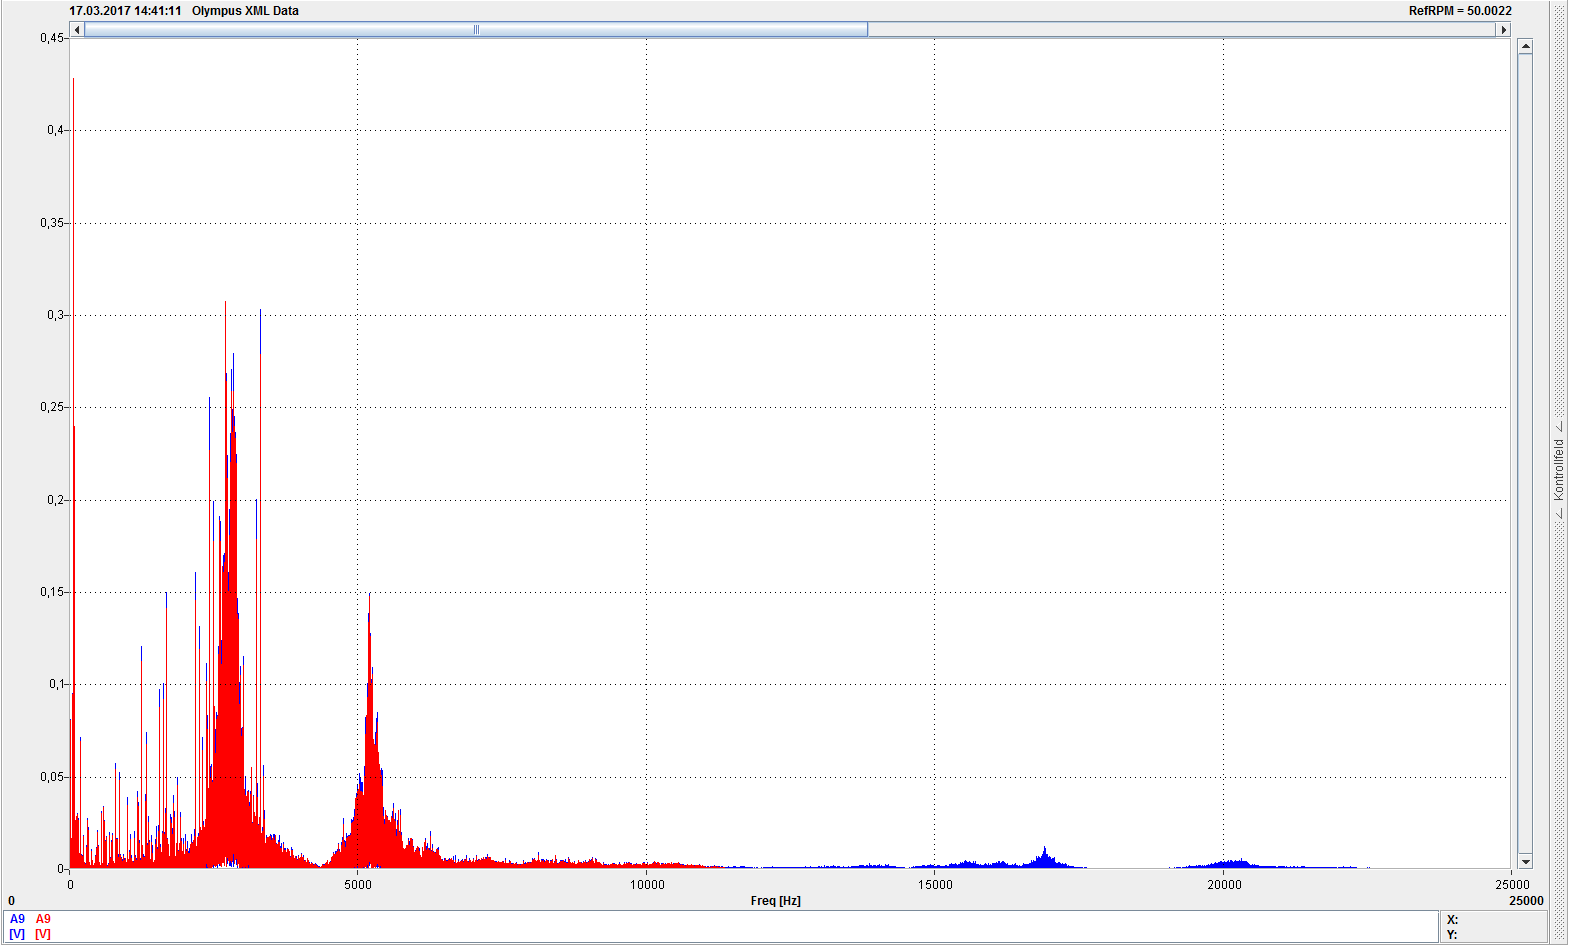
\includegraphics[width=0.49\textwidth]{Bilder/6.png}
				\caption{Qualitätslevel 5}
				\label{fig31}
			\end{varwidth}
			\begin{varwidth}[t]{\linewidth}
				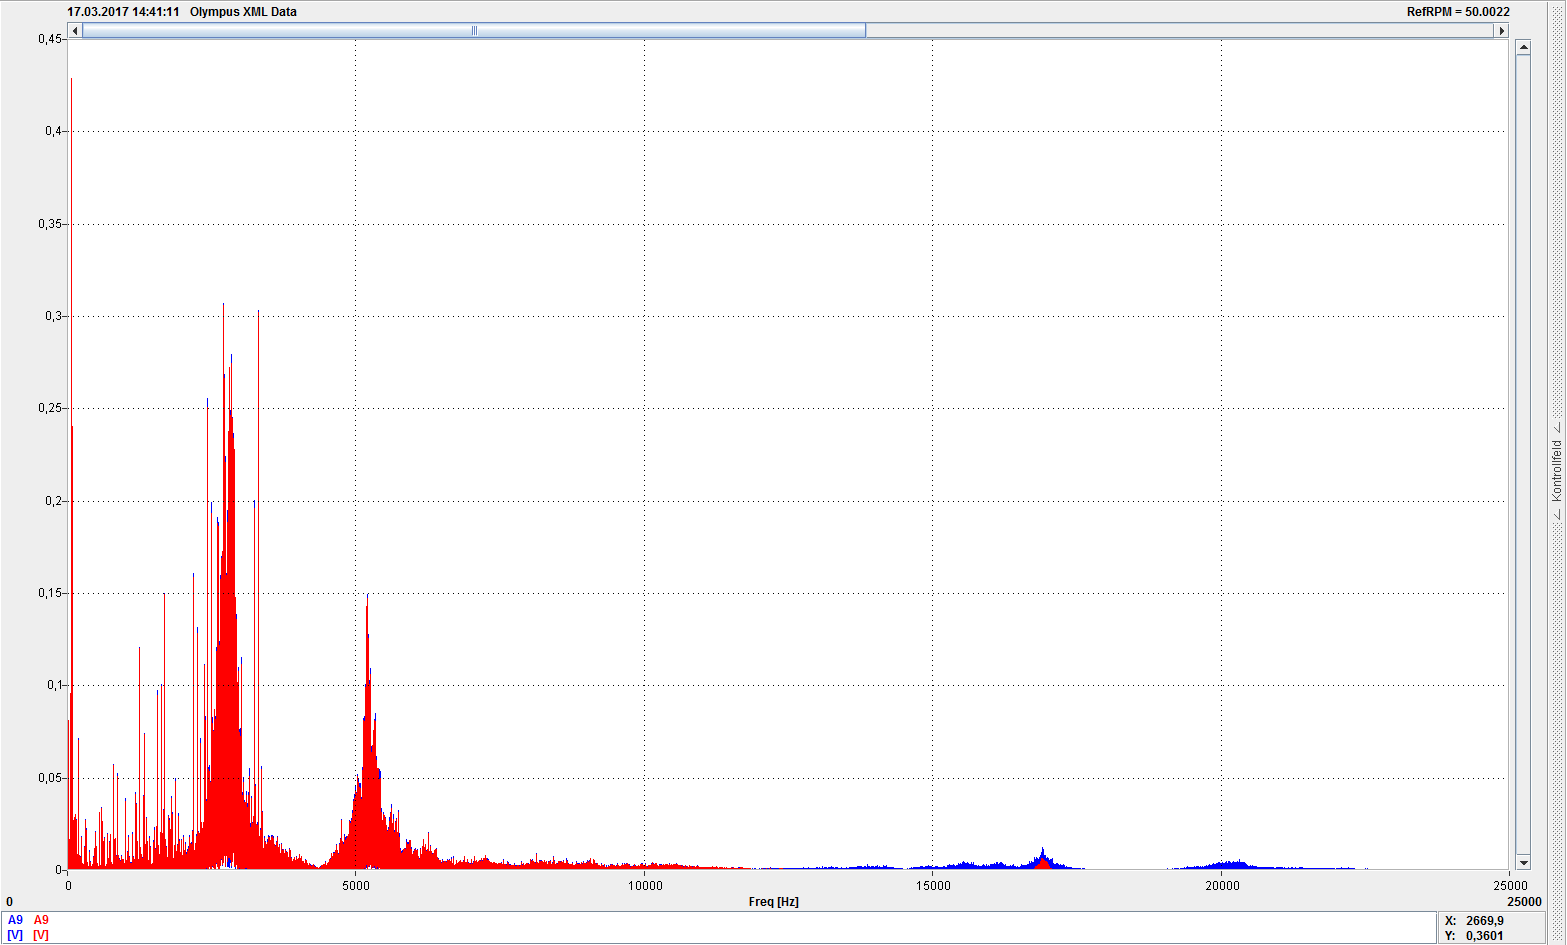
\includegraphics[width=0.49\textwidth]{Bilder/7.png}
				\caption{Qualitätslevel 9}
				\label{fig32}	
			\end{varwidth}
			\begin{varwidth}[t]{\linewidth}
				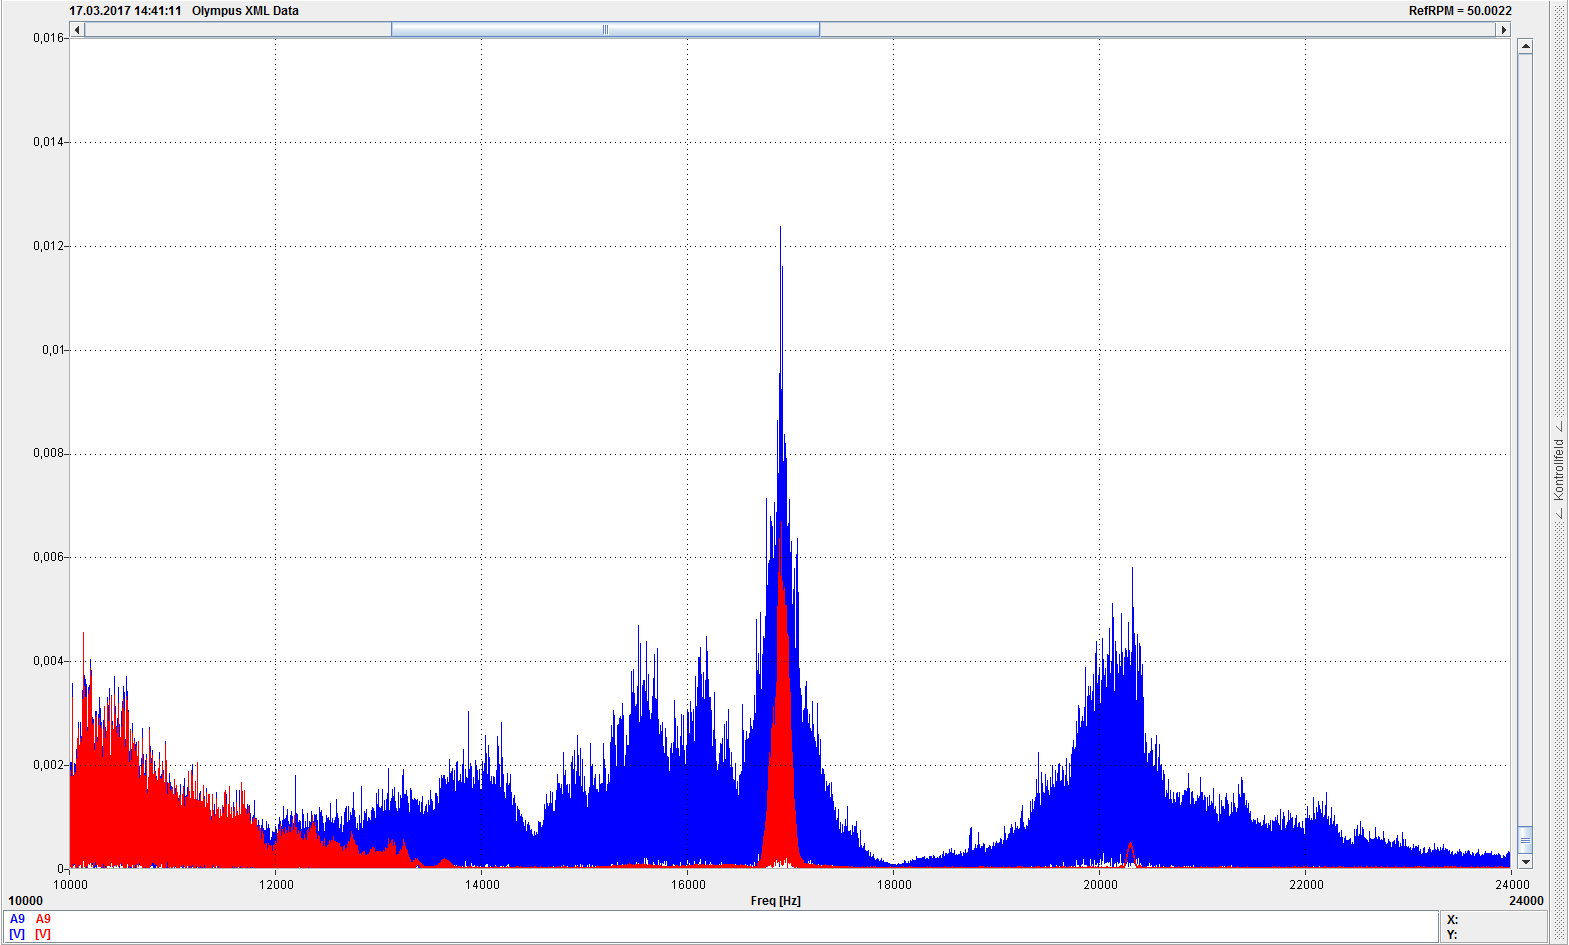
\includegraphics[width=0.49\textwidth]{Bilder/8.png}
				\caption{QL 9 bei hohen Frequenzen}
				\label{fig33}
			\end{varwidth}
				\begin{varwidth}[t]{\linewidth}
				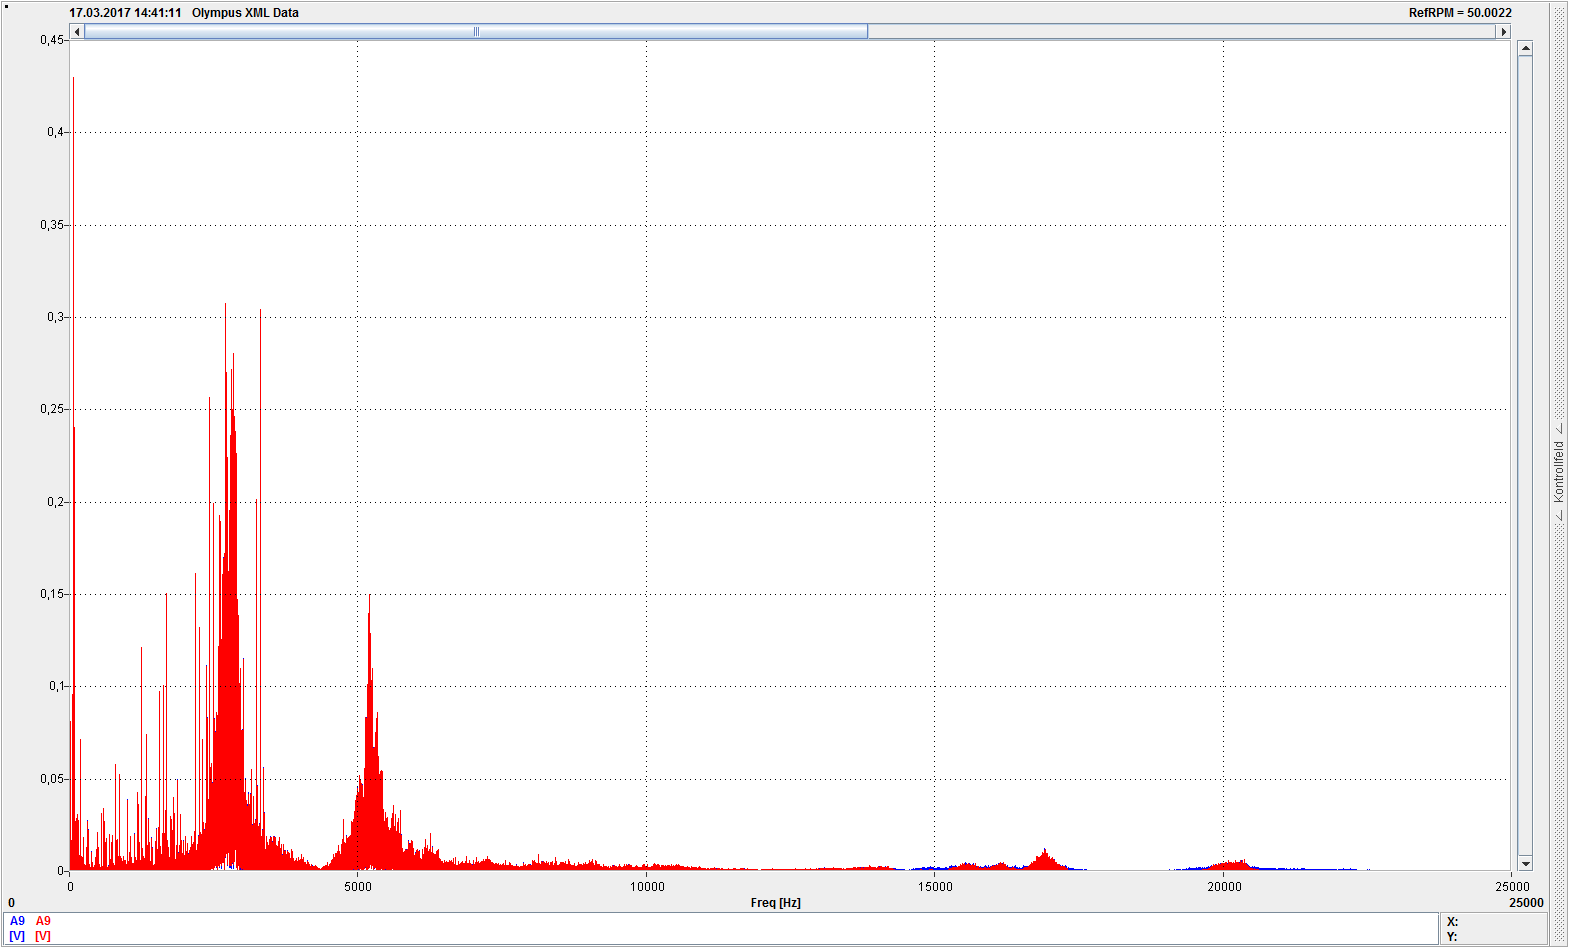
\includegraphics[width=0.49\textwidth]{Bilder/9.png}
				\caption{Qualitätslevel 10}
				\label{fig34}
			\end{varwidth}
			\begin{varwidth}[t]{\linewidth}
				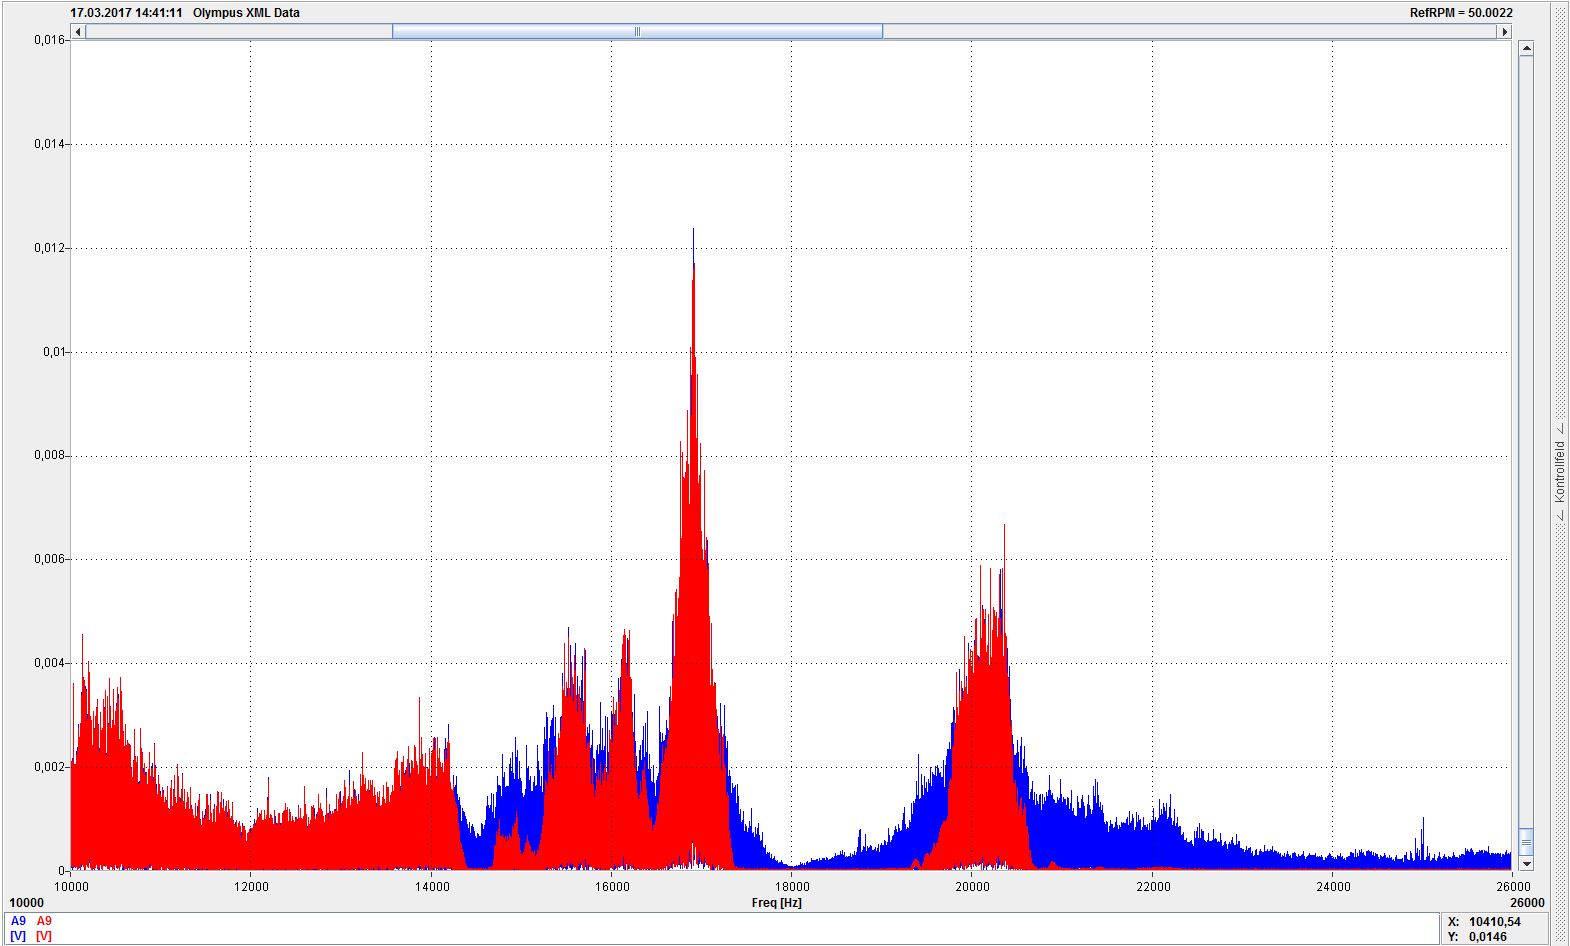
\includegraphics[width=0.49\textwidth]{Bilder/10.png}
				\caption{QL 10 bei hohen Frequenzen}
				\label{fig35}
			\end{varwidth}
		\end{figure}
		
			Die \textit{Abbildung \ref{fig12} - \ref{fig15} } zeigen die Zeitdaten (mV - s). In \textit{Abbildung \ref{fig12}} sind die unveränderten Originaldaten zu sehen.  Die darauffolgenden Abbildungen zeigen die Zeitdaten nach der Codierung und anschließender Encodierung bei verschiedenen Vorbis Qualitätsleveln. Bei einer niedrigen Qualität wie z.B. in \textit{Abbildung \ref{fig13}} ist eine deutliche Glättung der Kurve erkennbar, was einen Datenverlust mit sich bringt. Aber die Charakteristik der Kurve ist hier schon vorhanden. Bei der höchsten Qualität sind die Kurven bis auf ein paar Feinheiten nahezu identisch.
			
		\subsubsection{FFT Daten}
			Darstellung: In blau werden die Rohdaten dargestellt und rot die Enddaten.
			Bei einem Qualitätslevel von -1 (\textit{Abbildung \ref{fig30}}) kann man sehen, dass die Amplituden nicht immer dem Original entsprechen. Meistens sie diese zu klein. Außerdem ist auffällig, dass Frequenzen ab 90000 Hz vollkommen abgeschnitten sind.
			Ein Qualitätslevel von 5, wie in \textit{Abbildung \ref{fig31}}}, zeigt eine bessere Darstellung der Amplituden und dass die Frequenzen erst bei 11800 abgeschnitten werden.
			Bei Benutzung eines Qualitätslevels von 9 (\textit{Abbildung \ref{fig32}}) werden die Frequenzen nicht mehr komplett abgeschnitten. Hier wird das Verhältnis von Roh- und Enddaten langsam größer, bis die Frequenzen irgendwann erst einmal nicht mehr vorhanden sind. Dieser Prozess geht bei diesen Testdaten von 11800 Hz bis 13800Hz. Aber große Amplituden Maxima (z.B. bei 17000 Hz) werden nun trotzdem noch annäherungsweise dargestellt. Zu sehen in \textit{Abbildung \ref{fig33}}.
			Benutzt man, mit einem Qualitätslevel von 10, die beste Qualität, so sind die niedrigen Frequenzen nahezu identisch (\textit{Abbildung \ref{fig34}}). Ab ungefähr 14200Hz werden nur noch die Maxima dargestellt. Aber im Vergleich zu Level 9 werden auch schon kleinere Maxima dargestellt. Zwischen den Maxima werden jedoch die Frequenzen gedämpft. Zu sehen ist dies in \textit{Abbildung \ref{fig35}}.
		\subsubsection{Reduzierung}
			Die rohen Sensordaten können in einer .raw Datei abgelegt werden. Hierzu sind die Sensordaten in 32 Bit float Werten abgespeichert (ohne Header). Die .ogg Dateien besitzen einen Header, der ungefähr 1\% der Datenmenge beinhaltet.\\\\
			
			Reduzierung bei verschiedenen Qualitätslevel\\
			

			
			\begin{tabularx}{\textwidth}{p{0.25\textwidth}|l|l|l}
				Type 			& Größe in Bytes 		&  \\
				\hline
				.raw			& 5.242.880				& 100 \%		\\
				\hline
				\hline
				.ogg QL -1		& 52.579				& 1,002 \%\\
				\hline
				.ogg QL  5		& 121.202				& 2,311 \%	\\
				\hline
				.ogg QL 10		& 318.679				& 6,078 \%	\\
			\end{tabularx}
		

		
			Je nachdem welches Qualitätslevel gewählt wurde, hat das .ogg File nur noch 1 – 6 \% der ursprünglichen Daten.\\\\
			Reduzierung bei verschiedenen Datengrößen \\
			

			\begin{tabularx}{15cm}{p{0\textwidth}l|l|l|l|l}
				
				 &Messung& .raw Größe & ogg Größe & Verhältnis in \% \\
				 \hline
				 &1 &4.096 &3.457 & 84,399414 & \\
				 \hline
				 &2 &4.912 &3.615 & 73,595277 & \\
				 \hline
				 &3 &65.536 &14.366 & 21,920776 & \\
				 \hline
				 &4 &81.920 &14.742 & 17,995605 & \\
				 \hline
				 &5 &131.064 &20.009 & 15,266587 & \\
				 \hline
				 &6 &262.144 &33.043 & 12,604904 & \\
				 \hline
				 &7 &524.288 &32.530 & 6,2046051 & \\
				 \hline
				 &8 &1.152.000 &50.082 & 4,3473958 & \\
				 \hline
				 &9 &3.840.000 &157.990 & 4,1143229 & \\
				 \hline
				 &10 &5.242.880 &318.698 & 6,0786819 & \\
				 \hline
				 &11 &10.485.760 &560.778 & 5,3479958 & \\
				 \hline
				 &12 &15.728.640 &837.208 & 5,3228251 & \\
				 \hline
				 &13 &20.971.520 &1.115.197 & 5,3176737 & \\
				 
				 & & 
			\end{tabularx}
		
		\begin{figure}[h]
			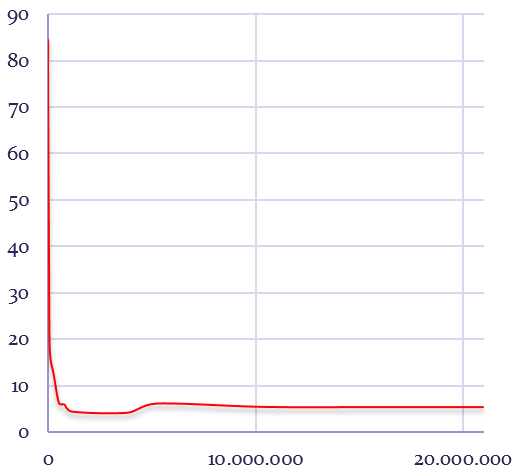
\includegraphics[scale=0.5]{Bilder/Capture1.png}
			\centering
			\vspace{0 cm}
			\caption{Reduzierung (Byte/\%)}
			\label{fig16}	
		\end{figure}
	
	Aus den Messungen lässt sich ablesen, dass der Vorbis Codec immer effektiver wird, umso größer die Rohdaten werden. Ein möglicher Grund dafür ist, dass der Header von jedem Vorbis Block immer die gleiche Größe hat. Die Auswirkung dieser Größe ist bei kleinen Dateien viel deutlicher als bei großen Dateien.
	Ab 500 kB kann man davon ausgehen, dass die OGG Größe 4-6\% der Rohdaten beträgt.
	Da die Vorbis Blöcke eine zufällige Seriennummer besitzen, kann die Größe der Dateien um einige Bytes abweichen!
		
\newpage			
	\subsection{Flac Komprimierung}	
		\subsubsection{Reduzierung}
		FLAC mit unterschiedlichen Qualitäten\\\\
		
		\begin{tabularx}{\textwidth}{p{0.25\textwidth}|l|l|l}
			Type 			& Größe in Bytes 		&  \\
			\hline
			.raw			& 5.242.880				& 100 \%		\\
			\hline
			\hline
			.flac QL 0		& 3.663.347				& 69,873 \%\\
			\hline
			.flac QL  8		& 3.653.476				& 69,685 \%	\\
			
		\end{tabularx}
	\\\\
	Nach der Komprimierung mit dem höchsten Kompressions Level hat die .flac Datei noch 69,685 \% der ursprünglichen Rohdaten.\\\\
	FLAC mit unterschiedlichen Datengrößen
	
				\begin{tabularx}{\textwidth}{p{0\textwidth}l|l|l|l|l}
		
		&Messung& .raw Größe & flac Größe & Verhältnis in \% \\
		\hline
		&1 &4.096 &2.740 & 66,89453 & \\
		\hline
		&2 &4.912 &3.532 & 71,90554 & \\
		\hline
		&3 &65.536 &46.863 & 71,50726 & \\
		\hline
		&4 &81.920 &41.219 & 50,31616 & \\
		\hline
		&5 &131.064 &98.427 & 75,09843 & \\
		\hline
		&6 &262.144 &153.860 & 58,69293 & \\
		\hline
		&7 &524.288 &267.630 & 51,04637 & \\
		\hline
		&8 &786.432 &322.681 & 41,03101 & \\
		\hline
		&9 &1.152.000 &640.059 & 55,56068 & \\
		\hline
		&10 &3.840.000 &1.331.625 & 34,67773 & \\
		\hline
		&11 &5.242.880 &3.653.476 & 69,68452 & \\
		\hline
		&12 &10.485.760 &4.370.038 & 41,67593 & \\
		\hline
		&13 &15.728.640 &6.875.124 & 43,71086 & \\
		\hline
		&14 &20.971.520 &8.826.739 & 42,08917 & \\
		
		& & 
	\end{tabularx}
	Bei einer Messung verschiedener Dateigrößen ergab sich eine Reduzierung von 40 -70\%. Umso größer die Dateien, umso größer wird die Reduzierung. Aber nicht so extrem wie bei Vorbis.\\
	Anmerkung: FLAC Dateien haben einen Header, .raw Dateien nicht (realer Wert wäre noch etwas kleiner).
	
		
	\subsection{Code}
	
		\begin{wrapfigure}[11]{r}[0pt]{0.5\textwidth}
			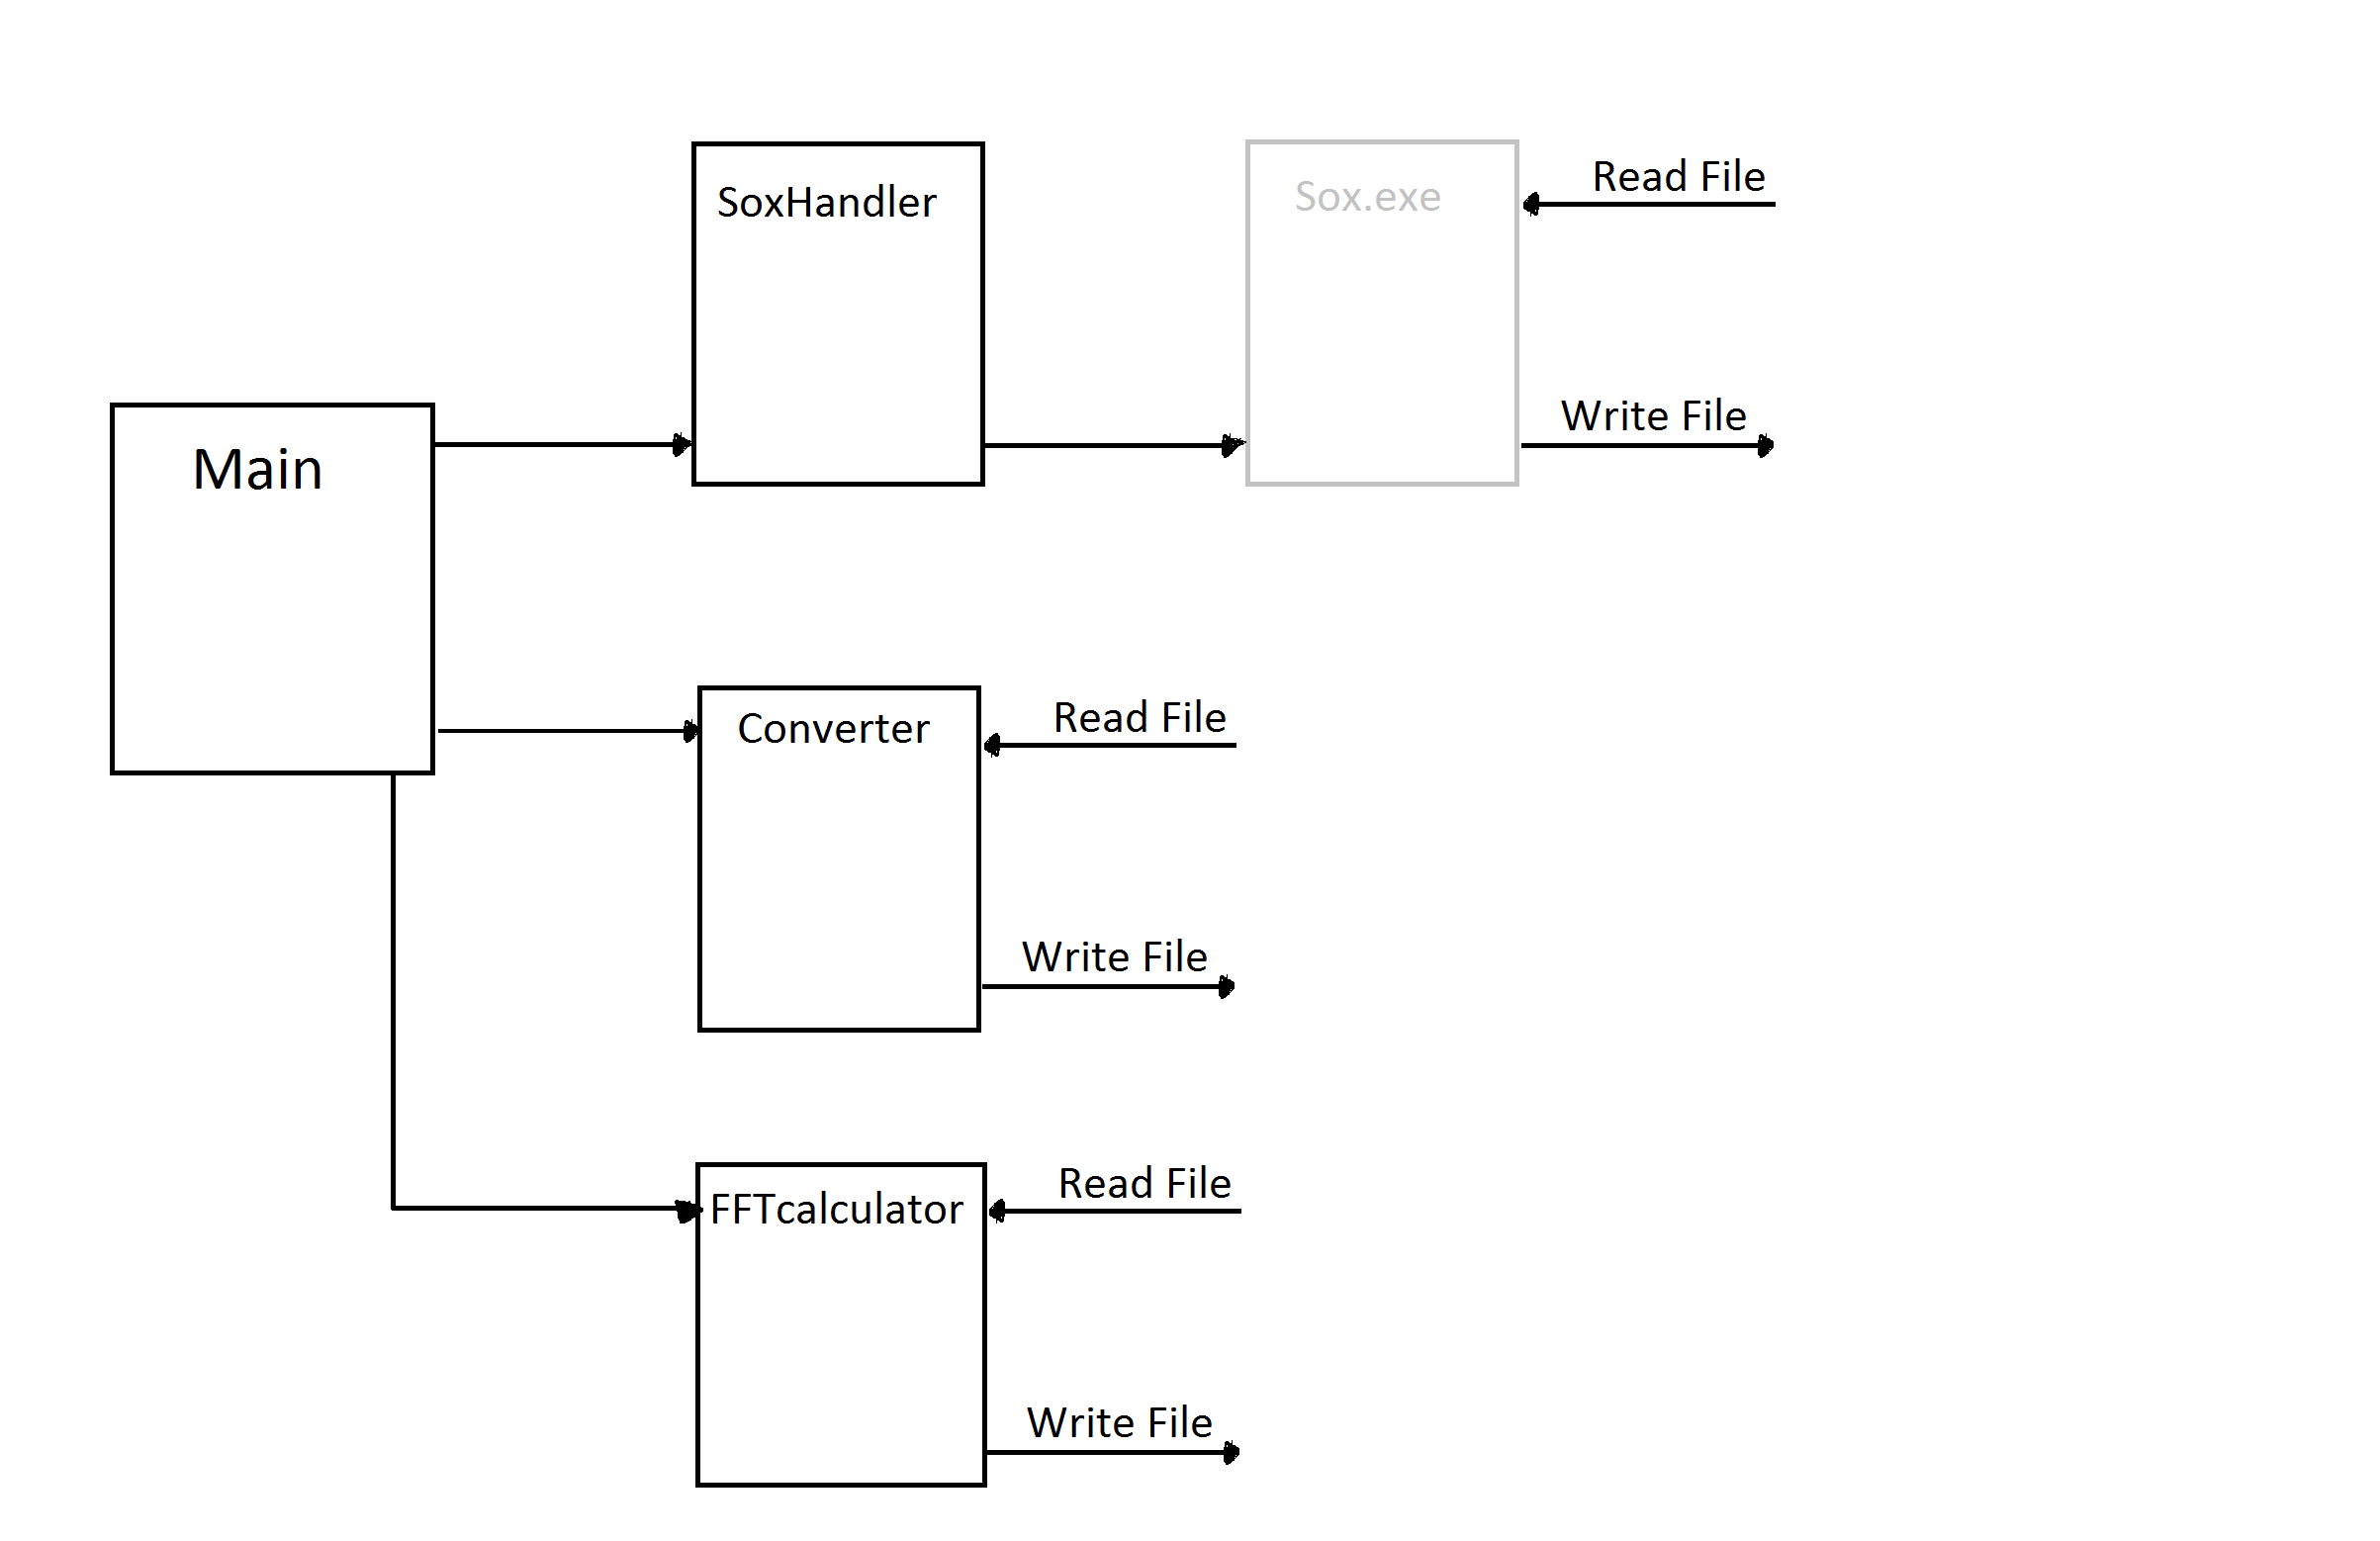
\includegraphics[scale=0.2]{Bilder/blockschaltbild1.png}
			\centering
			\vspace{0 cm}
			\caption{Code Struktur}
			\label{fig18}	
		\end{wrapfigure}
	
		\subsubsection{Struktur}
			Die Codestruktur ist wie in \textit{Abbildung \ref{fig18}} aufgebaut. Das Main Objekt hat Zugriff auf die anderen Objekte. Der SoxHandler öffnet die Sox.exe in der Konsole und gibt die Übergabeparameter weiter. SoX übernimmt die Kodierung und Dekodierung der Daten. Der Converter übernimmt die Umwandlung von Formaten ohne Kodierung. Mit Hilfe des FFTcalculator kann aus einer .raw Datei die FFT Daten berechnet werden.
			
			
		\subsubsection{Format Umwandlung}

			Das Projekt ist prinzipiell modular aufgebaut, das heißt, dass die Funktionen unabhängig voneinander funktionieren. So kann zum Beispiel ein anderes Start- oder Endformat gewählt werden. Unten (\textit{Abbildung \ref{fig19}}) zu sehen ist die maximale Ausdehnung des „Formatierungsbaums“. Dabei können vor und nach der Komprimierung FFT Daten berechnet werden, um den Unterschied zu erkennen.\\
			
			\begin{figure}[h]
				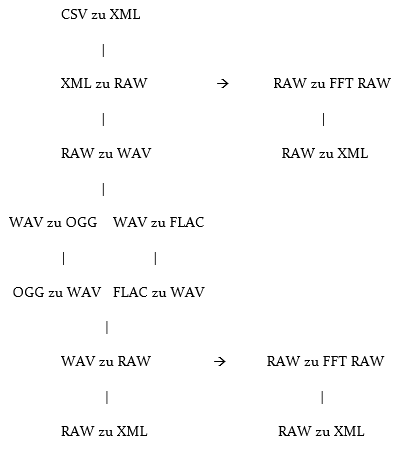
\includegraphics[scale=0.7]{Bilder/Capture2.PNG}
				\centering
				\vspace{0 cm}
				\caption{Format ,,Baum''}
				\label{fig19}	
			\end{figure}
				
	\subsection{Ergebnisse}
		Die mindestens 30\%ige Ersparnis der flac Codierung ist komplett ohne Auswirkungen anwendbar. Das einzige was hierzu benötigt wird ist Rechenleistung. Die Vorbis Codierung ist abhängig von der Dateigröße. Ab einer Dateigröße von ca. 500kB bringt sie eine Ersparnis von mindestens 90\%. Diese sehr hohe Komprimierung kostet aber Informationsgehalt in den oberen Frequenzen (ab ungefähr 12kHz).
		Alle verwendeten Codecs sind frei verfügbar und der Source Code des Encoders bzw. Decoders ist unter der Open Source Lizenz frei zugänglich.
		

\section{Projekt 3: Gerätekonfigurator über COM Port} 
	\subsection{Einleitung}
		\subsubsection{Motivation}
			Manchmal werden Geräte der Firma PRÜFTECHNIK vom Anwender falsch konfiguriert. Bei zum Beispiel falschen Netzwerkeinstellungen kann es sein, dass das Gerät nicht mehr erreichbar ist und so auch nicht über das Webfronend wieder repariert werden kann.
			Um das Gerät trotzdem wieder lauffähig zu machen, könne diese auch über eine serielle Schnittstelle (RS232) konfiguriert werden. Dies geschieht über eine Kommandoeingabe (wie zum Beispiel Putty).
			Da dies aber sehr unkomfortabel ist, wäre es schön den Vorgang durch eine GUI zu vereinfachen.
		\subsubsection{Aufgabe}
			Erstellen eines GUI Tools zum Wiederherstellen eines falsch konfigurierten Gerätes.
	\subsection{Benutzte Werkzeuge}
		\subsubsection{Eclipse}
			Eclipse ist eine freie Entwicklungsumgebung (IDE), die zur Programmierung mit vielen Sprachen eingesetzt werden kann. In diesem Projekt wurde sie zum Programmieren des Java Codes verwendet.
		\subsubsection{JavaFX}
			Framework zum Erstellen von Java Grafikoberflächen. Hier im Projekt wurde die Version 2.0 verwendet, damit es mit Java 1.7.0 kompatibel ist. Zum Einbinden in das Projekt wird ein Eclipse Plug-In (e(fx)clipse) verwendet.
		\subsubsection{Launch4J}
			Launch4j ist ein Open Source Tool, das es ermöglicht Java Anwendungen (.jar) in für Windows direkt ausführbare Dateien (.exe) umzuwandeln. Das heißt die Java Run Time wird von der .exe geöffnet. Dies hat den Vorteil, dass ausgesucht werden kann, welche Runtime verwendet werden soll. Ist diese nicht vorhanden kommt eine Installationsaufforderung. Außerdem ist es möglich eine Java Runtime mit dem Programm mitzuliefern, um komplett unabhängig von den installierten Runtimes zu sein.
		\subsubsection{Inno Setup}
			Inno Setup ist ein frei erhältliches Programm mit dem es möglich ist, ein Windows Installer zu erstellen. Dabei werden die gewünschten Konfigurationen und Einstellungen in einem .iss Skript festgelegt.\\\\
	\subsection{GUI}
	
		\begin{figure}
	
			\begin{varwidth}[t]{\linewidth}
				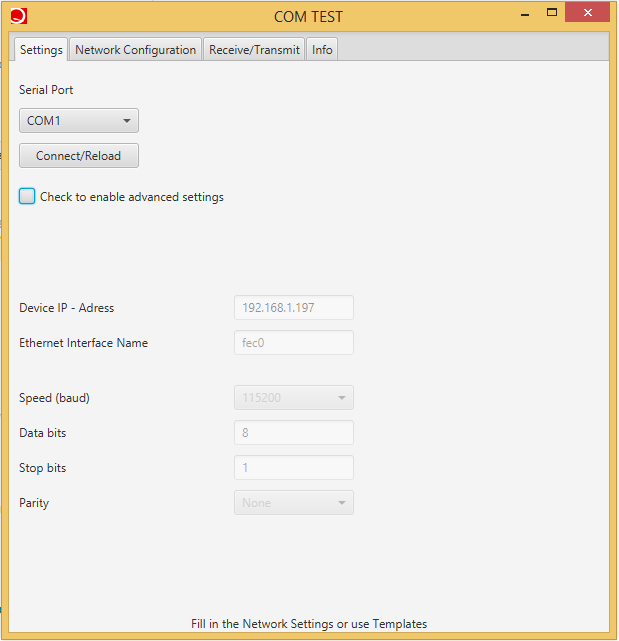
\includegraphics[width=0.49\textwidth]{Bilder/11.png}
				\caption{Start Seite mit Einstellungen}
				\label{fig40}	
			\end{varwidth} % ein Leerzeichen Abstand
			\begin{varwidth}[t]{\linewidth}
				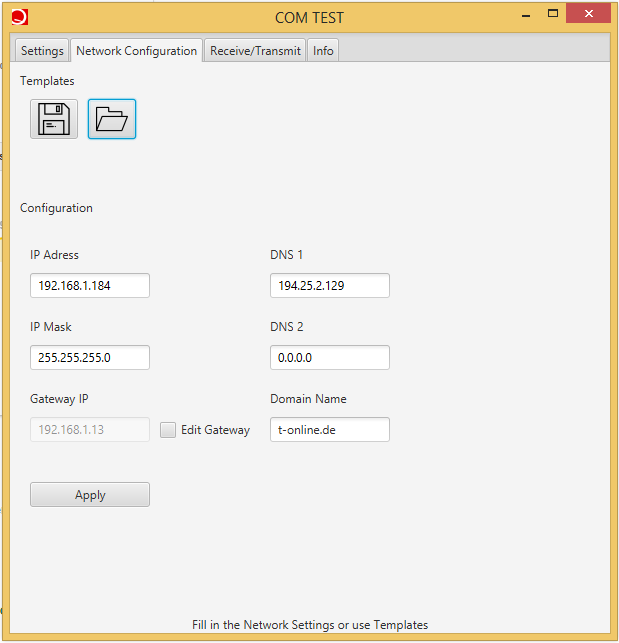
\includegraphics[width=0.49\textwidth]{Bilder/12.png}
				\caption{Netzwerkkonfiguration}
				\label{fig41}
			\end{varwidth}
			\begin{varwidth}[t]{\linewidth}
				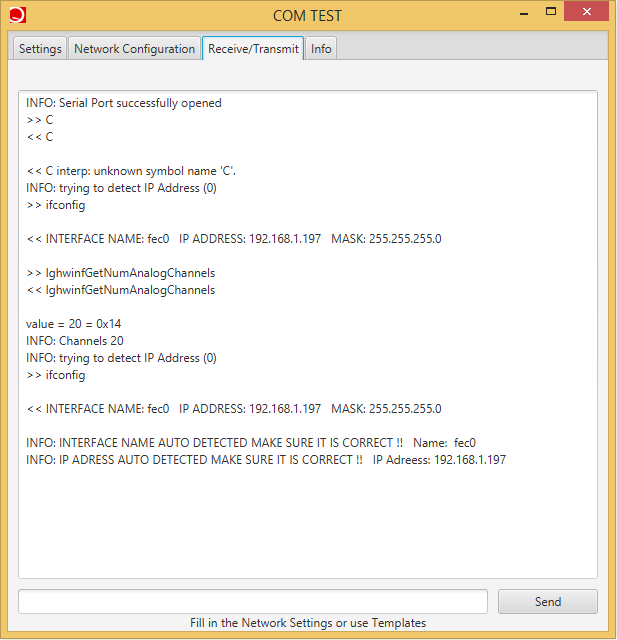
\includegraphics[width=0.49\textwidth]{Bilder/13.png}
				\caption{In / Output}
				\label{fig42}	
			\end{varwidth}
			\begin{varwidth}[t]{\linewidth}
				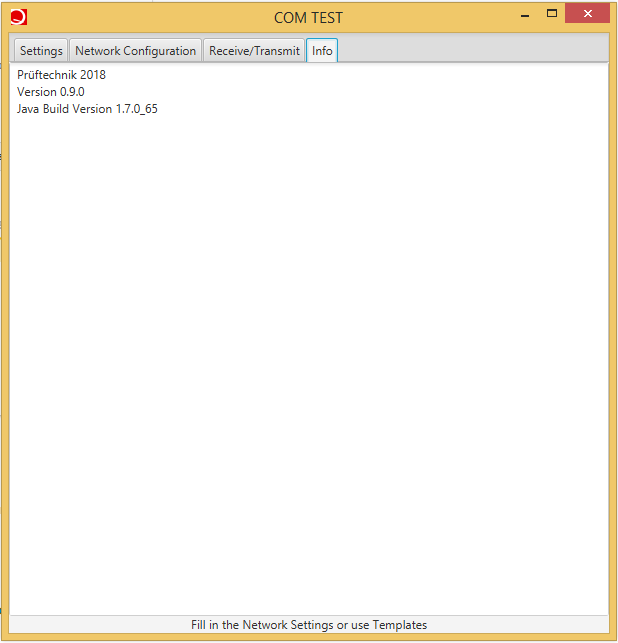
\includegraphics[width=0.49\textwidth]{Bilder/14.png}
				\caption{Info}
				\label{fig43}
			\end{varwidth}
		\end{figure}
	
		
		Auf \textit{Abbildung \ref{fig40}} ist der Tab für die Settings zu sehen. Dieser wird beim Starten der Anwendung aufgerufen, damit der Benutzer den gewünschten COM Port auswählen kann. Hat er dies gemacht und konnte die Verbindung erfolgreich hergestellt werden so wird der zweite Tab geöffnet (\textit{Abbildung \ref{fig41}}). Hier können dann die Netzwerkeinstellungen entweder von Hand oder durch die Benutzung eines Templates eingefügt werden. Durch das Drücken des „Apply“ Buttons werden die gewünschten Daten dann an das Gerät übertragen. Optional kann bei manchen Geräten auch noch die dauerhafte Speicherung ausgewählt werden. Dies ist aber nur möglich, wenn zudem noch eine Ethernet Verbindung besteht.
		Die seriellen Anfragen und Antworten sowie Info und Error Nachrichten können in dem Tab Receive/Transmit (\textit{Abbildung \ref{fig42}}) eingesehen werden.
	\subsection{Benutzung}
		Das Programm benötigt eine serielle Verbindung mit dem Gerät. Bei den VIBGUARD Modellen ist zusätzlich noch eine Ethernet Verbindung möglich, um die Einstellungen permanent zu speichern. 
		Sind zwei serielle Schnittstellen auf dem Gerät vorhanden sollte die RS232/2 Schnittstelle verwendet werden.
		WICHTIG: Es ist nicht möglich über die serielle Schnittstelle die Einstellungen dauerhaft zu speichern, aber es ist möglich die Einstellungen temporär zu setzen um ein falsch konfiguriertes Gerät wieder erreichbar zu machen und dann zum Beispiel über das Web Frontend die Einstellungen zu setzen. (Bei den VIBGUARD Modellen ist die Kommunikation mit dem Webserver ebenfalls implementiert)
		Vor Benutzung sollte das Gerät vollständig hochgefahren sein (System LED auf grün).
		Die aktuelle IP-Adresse und der Interface Name werden automatisch aus den Geräteantworten generiert und sollten auf Richtigkeit kontrolliert werden.
		Das Format der XML Templates ist wie folgt:\\\\\\
		

		<?xml version=''1.0'' encoding=''utf-8''?>\\
		<settings>\\
		<ipMask></ipMask>\\
		<ipGateway></ipGateway>\\
		<dns1></dns1>\\
		<dns2></dns2>\\
		<domainName> </domainName>\\
		</settings>\\\\
		Kann aber vom Programm automatisch generiert werden!
		
	\subsection{Code}
		Der Code ähnelt dem Model-View-Controller Prinzip. Zentral ist die Controller Klasse, die den Umgang mit den wichtigsten Objekten beinhaltet.
		\subsubsection{Struktur}
		\begin{figure}[h]
			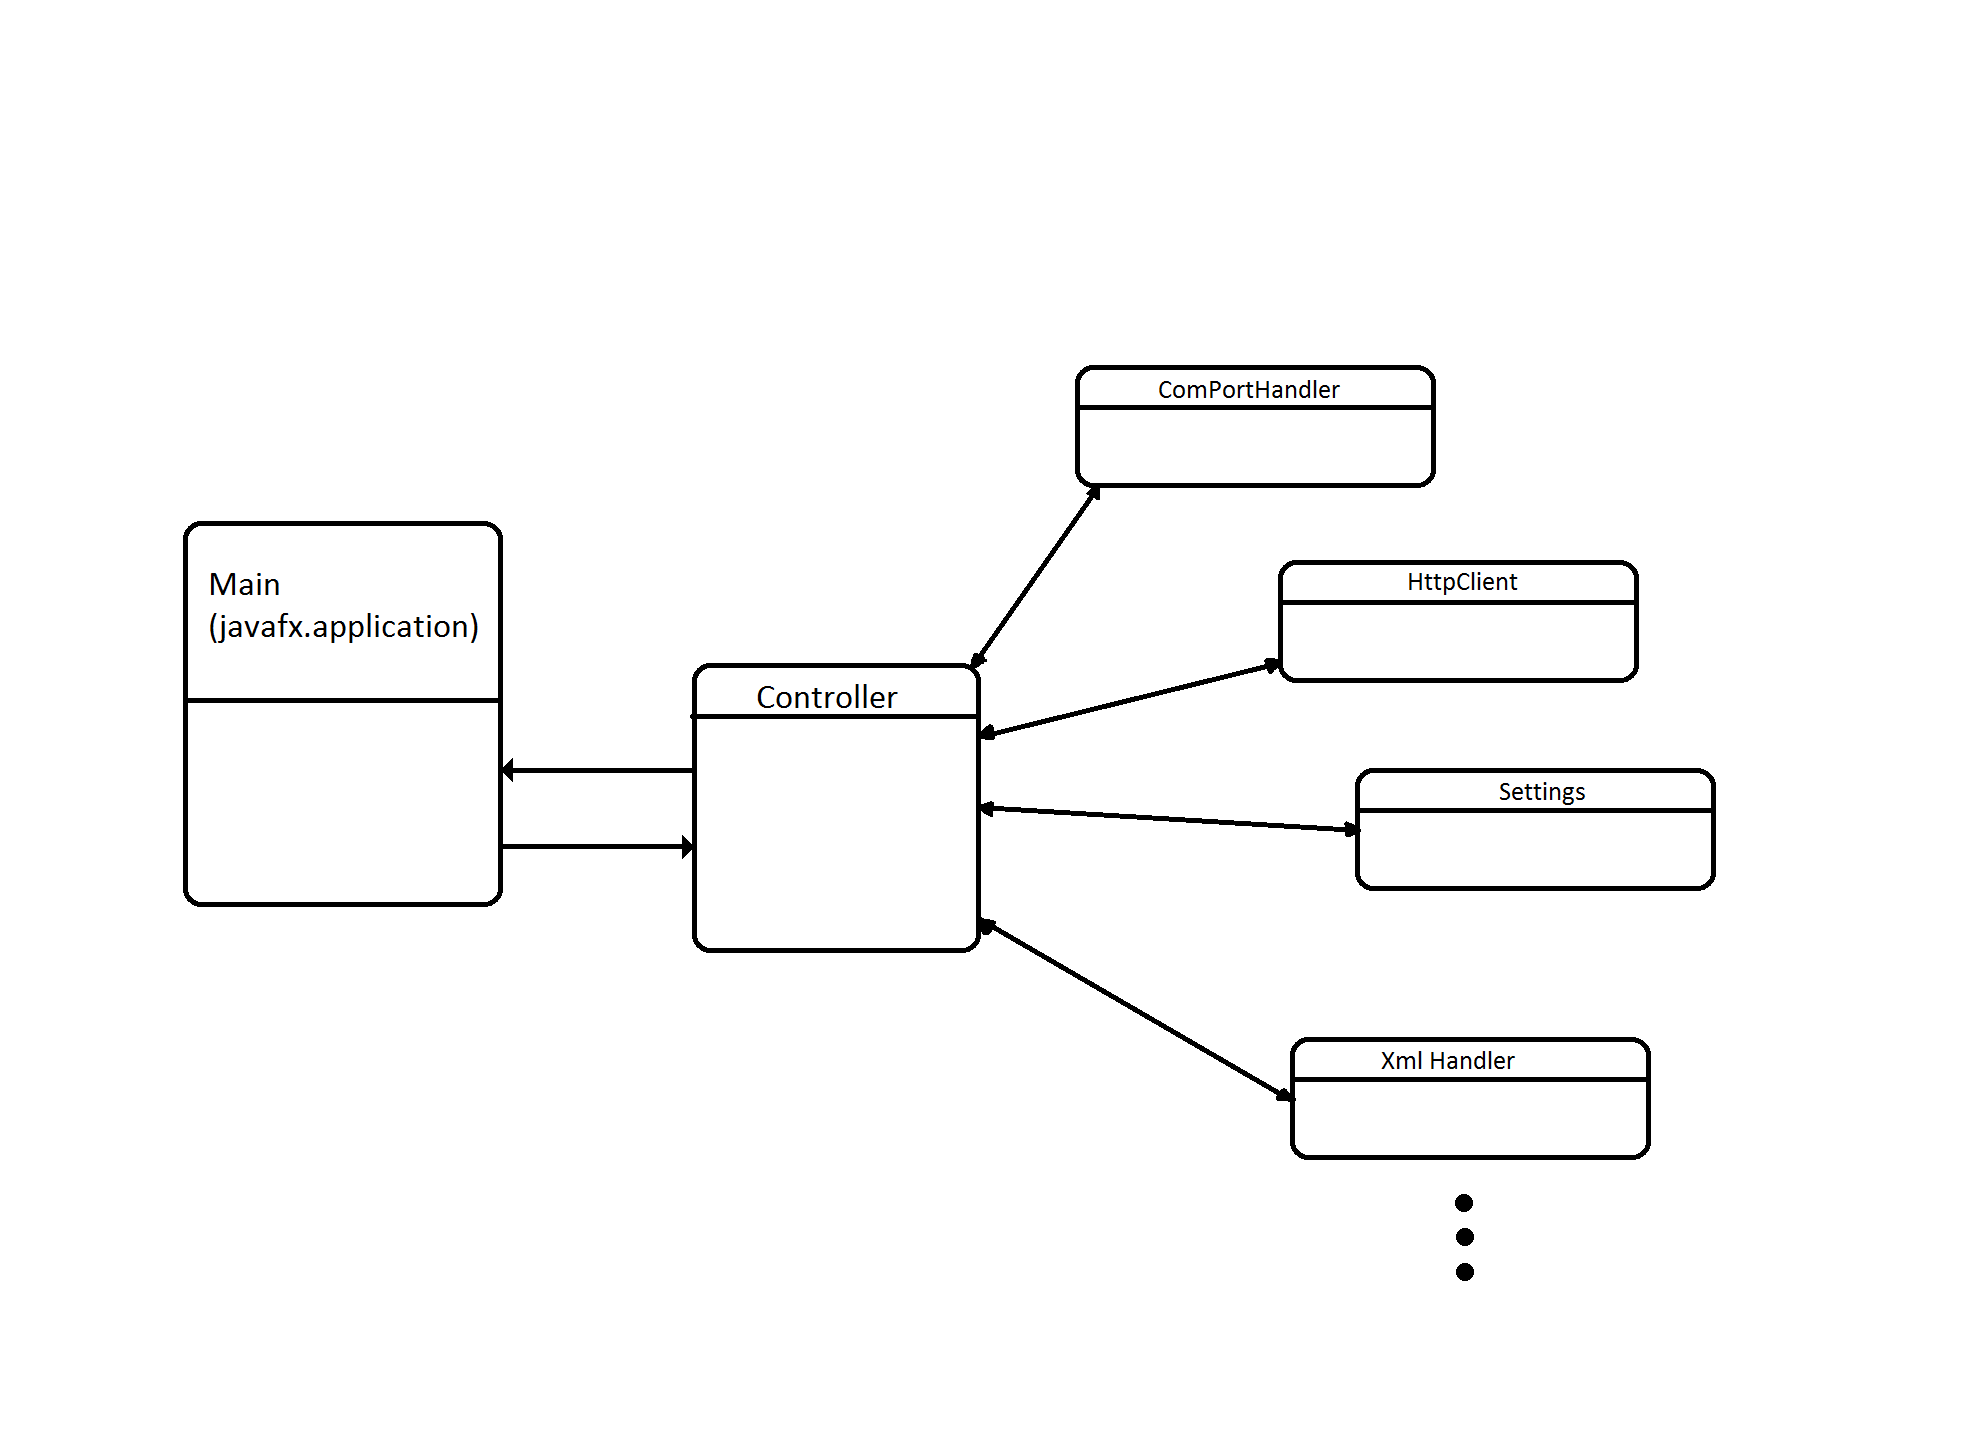
\includegraphics[scale=0.3]{Bilder/comuml.png}
			\centering
			\vspace{0 cm}
			\caption{Code Aufbau}
			\label{fig20}	
		\end{figure}
		\subsubsection{Eingebundene Bibliotheken}
		
		\begin{description}
			\item[RXTX Comm]
					ist eine Bibliothek, die es möglich macht mit Java auf eine serielle oder parallele Schnittstelle zu schreiben aber sie auch auszulesen. Dabei werden über die JNI native Treiber eingebunden. Wurde hier dazu verwendet, um über die serielle Schnittstelle zu kommunizieren.
			\item[Apache HttpClient] 
					macht es möglich mit Java http Anfragen an einen Webserver zu senden und die Antwort auszuwerten. In diesem Projekt wurde er dazu verwendet um mit dem Webserver des Devices zu kommunizieren, um ggf. die Netzwerkeinstellungen permanent zu speichern.
			\item[Jsoup] 
					ist ein HTML Parser, der aus einer HTML Datei einen DOM generiert und sie somit auslesbar macht. Wird hier verwendet, um aus der http Antwort des Device Webservers die derzeitigen Netzwerkeinstellungen auszulesen.
			\item[Apache Addressvalidator]
					ist eine Bibliothek, die IP Adressen auf ihre Richtigkeit (Gültigkeit) überprüft.
		\end{description}
		
\section{Projekt 4: WebApp: Return of Investment} 
	\subsection{Aufgabenstellung/Motivation}
		PRÜFTECHNIK stellt Messgeräte her, die dazu dienen eine beliebige Pumpe und den dazugehörigen Antrieb richtig auszurichten. Dies hat den Vorteil, dass der Wirkungsgrad und die Ausfall- bzw. Wartungswahrscheinlichkeit verbessert wird.
		Beim Verkauf und Marketing wird ein ROI (Return of Investment) Rechner verwendet, um dem Kunden die Ersparnis, die durch den Kauf des Produktes entstehen würde, zu verdeutlichen und ihn zum Kauf zu animieren.
		Dieser Rechner war in den letzten Jahren in Form einer Webseite realisiert, die jedoch nicht auf die Benutzung auf Smartphones/ Tablets ausgelegt ist.
		Die Aufgabe ist es nun diesen Rechner als Webapp zu realisieren, die auch auf kleinen sowie großen Bildschirmen (Responsive UI) gut funktioniert.
	\subsection{Materialien und Methoden}
		\subsubsection{NPM}
		NPM (Node Package Manager) ist ein Paketmanager, der es ermöglicht JavaScript Pakete herunterzuladen und zu verwalten. Die Verwaltung übernimmt eine JSON Datei, in die die gewünschten Pakete eingetragen werden.
		Pakete die mit Hilfe von npm eingebunden werden sind zum Beispiel React.js und Material UI.
		\subsubsection{React.js}
		React.js ist eine JavaScript Bibliothek zur Erstellung von Benutzeroberflächen. Veröffentlicht wurde React 2013 von Facebook (Open Source). Ein großer Vorteil von React ist der „Virtuelle DOM Baum“, der es möglich macht nicht immer den kompletten DOM zu rendern. Um das DOM zu erstellen werden ihm React Komponenten hinzugefügt.
		Eine React Komponente besitzt immer eine render() Funktion, die meistens eine JSX Struktur zurückgibt. Diese Strukturen werden dann später als Webseite dargestellt.
		\subsubsection{React Material UI}
		Material UI beinhaltet die UI Elemente (Buttons; Textfelder …), die im Stil von Googles eigenem Design (Material Design) erstellt sind. Die Elemente können dann als React Komponenten dem DOM hinzugefügt werden.
		Vorteil bei Material UI ist, dass es in der Lage ist eine „Responsive“ WebApp zu erstellen, die sich auf fast alle Displaygrößen anpassen kann.
		\subsubsection{JSX}
		JSX ist eine Syntax Erweiterung zu JavaScript und wird verwendet, um den Aufbau des User Interfaces zu definieren. Dabei ist sie XML ähnlich aufgebaut, mit eingebettetem JavaScript Code. 
		\subsubsection{Redux}
		Redux ist ein Framework mit dem man auf einfache Art den Status (Variablen, Werte…) verwalten kann. Zudem macht es so die Kommunikation zwischen verschiedenen React Komponenten möglich.\\
		Zentral ist der Redux Store, dem alle zu teilenden Werte hinzugefügt werden.
		\subsubsection{Hash Router}
		React erzeugt eine Single-Page App/Webseite. Dies ist möglich, da durch den virtuellen DOM bei Änderungen nicht die komplette Seite neu geladen werden muss. Dies hat jedoch den Nachteil, dass die „vor und zurück“ Buttons im Browser nicht funktionieren – da man keine andere Seite hat auf die man wechseln kann. Außerdem hat die Seite immer die gleiche URL. 
		Der Hash Router ermöglicht es, abhängig von der URL, eine andere React Komponente zu rendern. So wird eine Multipage App simuliert. 
		\subsubsection{Webpack}
		Webpack macht es möglich aus vielen JavaScript Dateien eine große zu generieren. Dies ist vor allem bei der Benutzung von npm nützlich, da hier viele kleine Dateien entstehen, die man sonst alle einzeln ausliefern müsste.
		Zusätzlich ist Webpack in der Lage, die Dateigröße um ein Vielfaches zu reduzieren in dem unnötiger Text wie Tabs, Kommentare oder Leerzeichen rausgenommen werden. Außerdem reduziert Webpack die Größe durch Ändern der Variablen- und Funktionsnamen auf zum Beispiel nur ein Zeichen. Der Code ist aber danach für den Menschen fast nicht mehr lesbar.
		\subsubsection{Babel.js}
		Ist ein JavaScript Compiler der die neueste ES 6 (ECMAScript) Version in eine alte, für alle Browser kompatible, Version umwandelt (meistens ES 5). 
		\subsubsection{Visual Studio Code}
		Visual Studio Code ist der hier verwendete Text Editor für die JavaScript Entwicklung. Vorteil hierbei ist die bereits eingebaute Konsole im Editor.
		\subsubsection{Google Chrome}
		Als Browser wurde Google Chrom verwendet. Vorteil hierbei sind die von Haus aus eingebauten Entwicklertools.
	\subsection{Vorlage/ Original}
	

	Die originale Seite, die als Vorlage dient, ist in \textit{Abbildung \ref{fig21}} zu sehen. Sie ist eine reine Desktopanwendung und kann den jährlichen Verlust bei einer Maschinenfehleinstellung berechnen. Dabei werden die Kosten in Energiekosten, Dichtungskosten, Kugellagerkosten und Pumpenreparationskosten eingeteilt. Im Layout hat jeder Kostenbereich einen eigenen Tab bekommen.
	Über diverse Textfelder und Eingabemöglichkeiten lassen sich hier die maschinenspezifischen Werte eintragen. Die entstehenden Gesamtkosten werden immer unten im Bildschirm angezeigt. Durch einen zusätzlichen Reiter im oberen Bildschirmrand lässt sich zusätzlich ein „Best Case“ Beispiel anschauen, um das mögliche Potential anzuzeigen.
	

	
	\begin{figure}[h]
		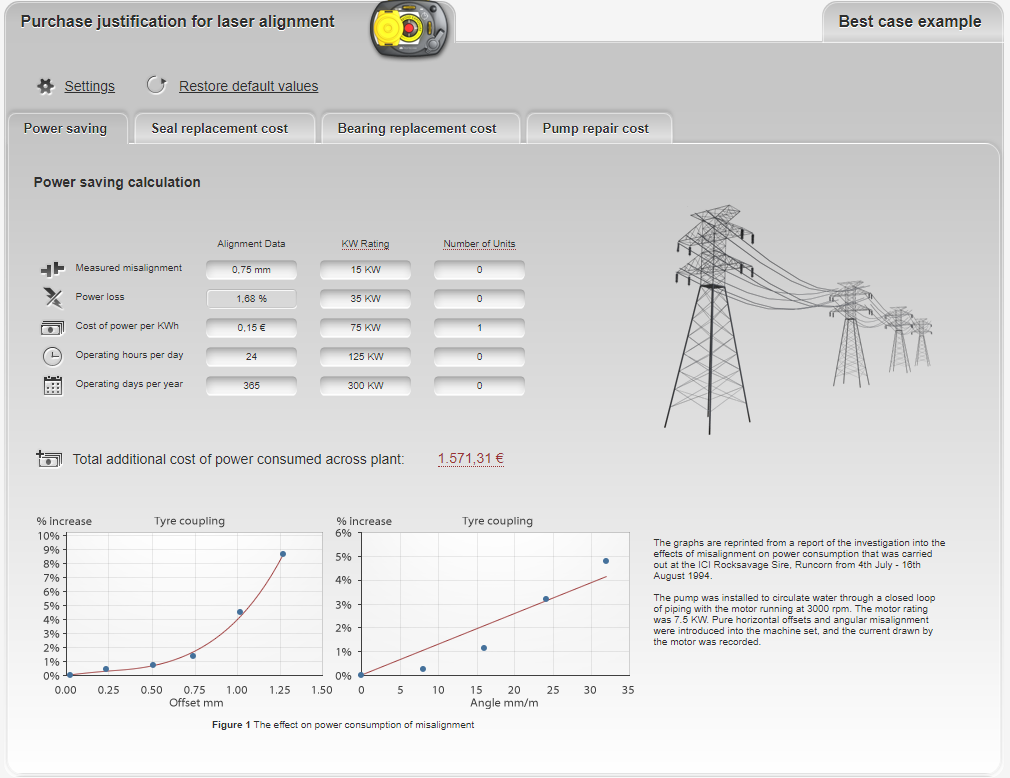
\includegraphics[scale=0.5]{Bilder/15.png}
		\centering
		\vspace{0 cm}
		\caption{Original Website}
		\label{fig21}	
	\end{figure}

	\newpage
	\subsection{Ergebnisse}
	
	
		\subsubsection{User Interface}
		
		
			\begin{wrapfigure}[45]{r}[0pt]{0.4\textwidth}
				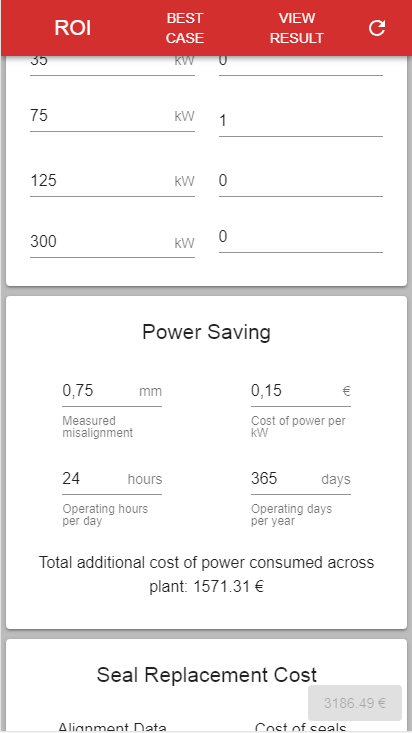
\includegraphics[scale=0.38]{Bilder/16.png}
				\centering
				\vspace{0 cm}
				\caption{Startseite}
				\label{fig22}	
				
				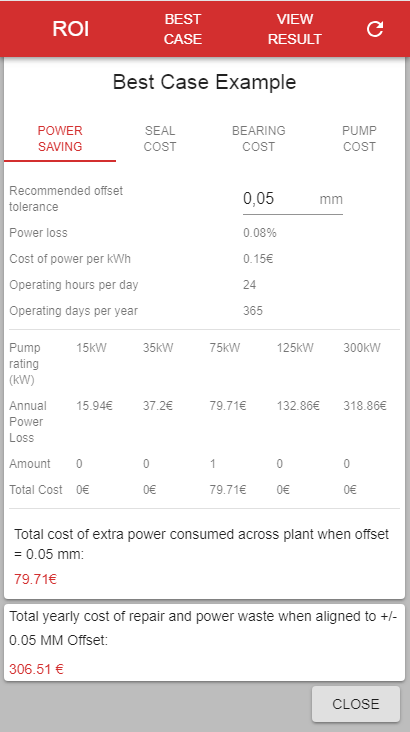
\includegraphics[scale=0.38]{Bilder/17.png}
				\centering
				\vspace{0 cm}
				\caption{Best Case Anzeige}
				\label{fig23}	
				
				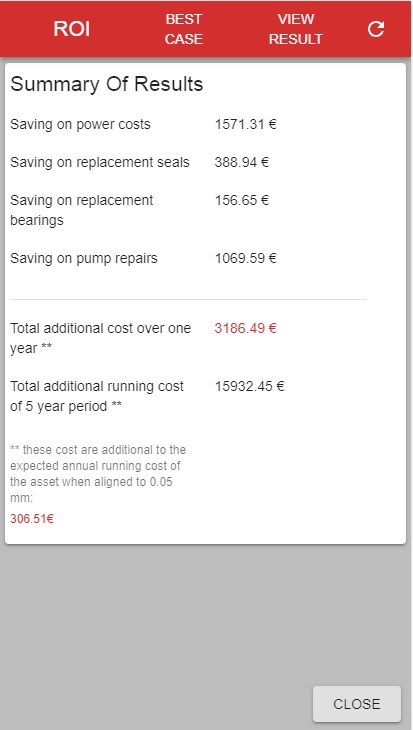
\includegraphics[scale=0.38]{Bilder/18.png}
				\centering
				\vspace{0 cm}
				\caption{Ergebnis Zusammenfassung}
				\label{fig24}
				
			\end{wrapfigure}
			
		
			Die Hauptseite (\textit{Abbildung \ref{fig22}}) zeigt die einzelnen Cards in die man die spezifischen Eingaben eintragen kann und die dazugehörigen Werte berechnet werden. Das benutzte Grid Layout ist in der Lage sich auf die einzelnen Displaygrößen anzupassen.
			Die AppBar ist am oberen Bildschirm fixiert und bleibt auch beim Scrollen erreichbar. Die Buttons in der AppBar können dazu verwendet werden um zu den zwei anderen Ansichten (BEST CASE und VIEW RESULT) zu wechseln. Im unteren Bereich werden zusätzlich die jährlichen Gesamtkosten angezeigt.

			In der Ansicht „Summery of Results“ (\textit{Abbildung \ref{fig23}}) werden die jährlichen Kosten der einzelnen Gebiete angezeigt und zusammengerechnet.

			Die „Best Case Example“ Ansicht (\textit{Abbildung \ref{fig24}}) zeigt, wie viel Kosten entstehen würden, wenn die Maschine korrekt ausgerichtet ist. Außerdem wird auch die Zusammensetzung des Ergebnisses angezeigt.\\
			Ein Tab Menü macht es möglich die Kosten der verschiedenen Bereiche einzusehen.\\\\
			

	\subsection{Code}
		\subsubsection{JavaScript}
			Wie oben beschrieben baut der JavaScript Code auf das React Framework auf. Daher ist das Root Element (Objekt) der ReactDOM. Direkt danach wir mit Hilfe eines Providers der REDUX Store hinzugefügt.
			Außerdem kommt eine MuiThemeProvider zum Einsatz, der das Theme (Farbtabelle) für die Material UI Komponenten definiert.
			Danach folgt die Definition des User Interfaces mit Hilfe verschiedener React Komponenten, die mit Hilfe von JSX arrangiert werden.
			Nach der App Bar wird dann der Hash Router eingebaut, um den Inhalt abhängig von der URL zu machen.
			Zusätzlich sind diverse Funktionen implementiert, die die ROI Werte berechnen und ausgeben. Diese wurden aus der JavaScript Datei der Vorlage entnommen.
		\subsubsection{HTML}
			Da fast der komplette DOM Baum über JavaScript und React aufgebaut ist, fällt der HTML Code eher klein aus. Das einzige das React im HTML Body benötigt, ist ein Root <div> Tag und das Einbinden der JavaScript Datei.
			Um aber die WebApp für jedes Gerät und möglichst auch offline benutzbar zu machen sind zudem noch diverse Features hinzugefügt.
			Zum Beispiel wird ein HTML Manifest, WebApp Manifest und Icons für ein breites Spektrum an Geräten eingebauut.
		\subsubsection{CSS}
			Auf CSS wurde komplett verzichtet, da der Style der Komponente auch direkt in JSX eingebunden werden kann.
		
\section{Quellenverzeichnis}

https://developer.android.com/studio/index.html\\
https://www.pruftechnik.com/\\
https://de.wikipedia.org/wiki/Android\_(Betriebssystem)\\
https://de.wikipedia.org/wiki/Android\_Studio\\
http://www.programmierenlernenhq.de/tutorial-android-activities-und-intents/\\
https://de.wikipedia.org/wiki/Gradle\\
https://developer.android.com/reference/android/media/AudioRecord.html\\
http://www.android-graphview.org/\\
https://de.wikipedia.org/wiki/Schnelle\_Fourier-Transformation\\
https://de.wikipedia.org/wiki/Puls-Code-Modulation\\
https://de.wikipedia.org/wiki/Ogg\\
https://de.wikipedia.org/wiki/Vorbis\\
https://de.wikipedia.org/wiki/Modifizierte\_diskrete\_Kosinustransformation\\
https://de.wikipedia.org/wiki/Free\_Lossless\_Audio\_Codec\\
http://sox.sourceforge.net/sox.html\\
https://de.wikipedia.org/wiki/CSV\_(Dateiformat)\\
https://de.wikipedia.org/wiki/Extensible\_Markup\_Language\\
https://de.wikipedia.org/wiki/Eclipse\_(IDE)\\
https://de.wikipedia.org/wiki/JavaFX\\
http://launch4j.sourceforge.net/\\
http://www.jrsoftware.org/isinfo.php\\
http://rxtx.qbang.org/wiki/index.php/FAQ\\
https://hc.apache.org/httpcomponents-client-ga/\\
https://jsoup.org/\\
https://commons.apache.org/proper/commons-validator/apidocs/org/apache/commons/validator/routines/InetAddressValidator.html\\
https://de.wikipedia.org/wiki/NPM\_(Software)\\
https://reactjs.de/artikel/react-tutorial-deutsch/\\
https://material-ui.com/\\
https://reactjs.org/docs/introducing-jsx.html\\
https://medium.freecodecamp.org/beginners-guide-to-react-router-4-8959ceb3ad58\\

\section{Abbildungsverzeichnis}
https://cdn-images-1.medium.com/max/523/1*BmgNxyQaWUflgZDK96i9cg.png



\end{document}

